\documentclass{article}
\usepackage{amsmath, amssymb, kotex, hyperref, graphicx, mdframed, setspace,enumitem}
\usepackage[a4paper, margin = 40pt]{geometry}
\setstretch{1.5}
\begin{document}
\title{시계열 회귀분석(Time Series Regression - 3)}
\author{강의 : 김성범 교수님\\ 정리 :  김선중}
\date{\today}
\maketitle

이것은 \href{https://youtu.be/5QnR4L3KGz4}{Time Series Regression - Part 3} 강의에 대한 노트이다.
\tableofcontents

\bigskip\bigskip
%\newpage
아래 식에서 보듯이, 많은 경우에 시계열은 추세(trend)와 계절성(seasonality), 그리고 오차로 이루어져있다.
이번 강의에서는 seaonsal variation을 모델링하는 네 가지 모델에 대해서 다루는 것 같다.
그것들은
\begin{itemize}[itemsep=0pt,parsep=0pt]
\item
binary variable models
\item
trigonometric models
\item
growth curve models
\item
first-order autoregressive process
\end{itemize}
이다.
이 중에서 앞의 세 개는 고전적인 방법이고 마지막 방법이 앞으로 계속 사용할 방법인 것 같다.

\begin{center}
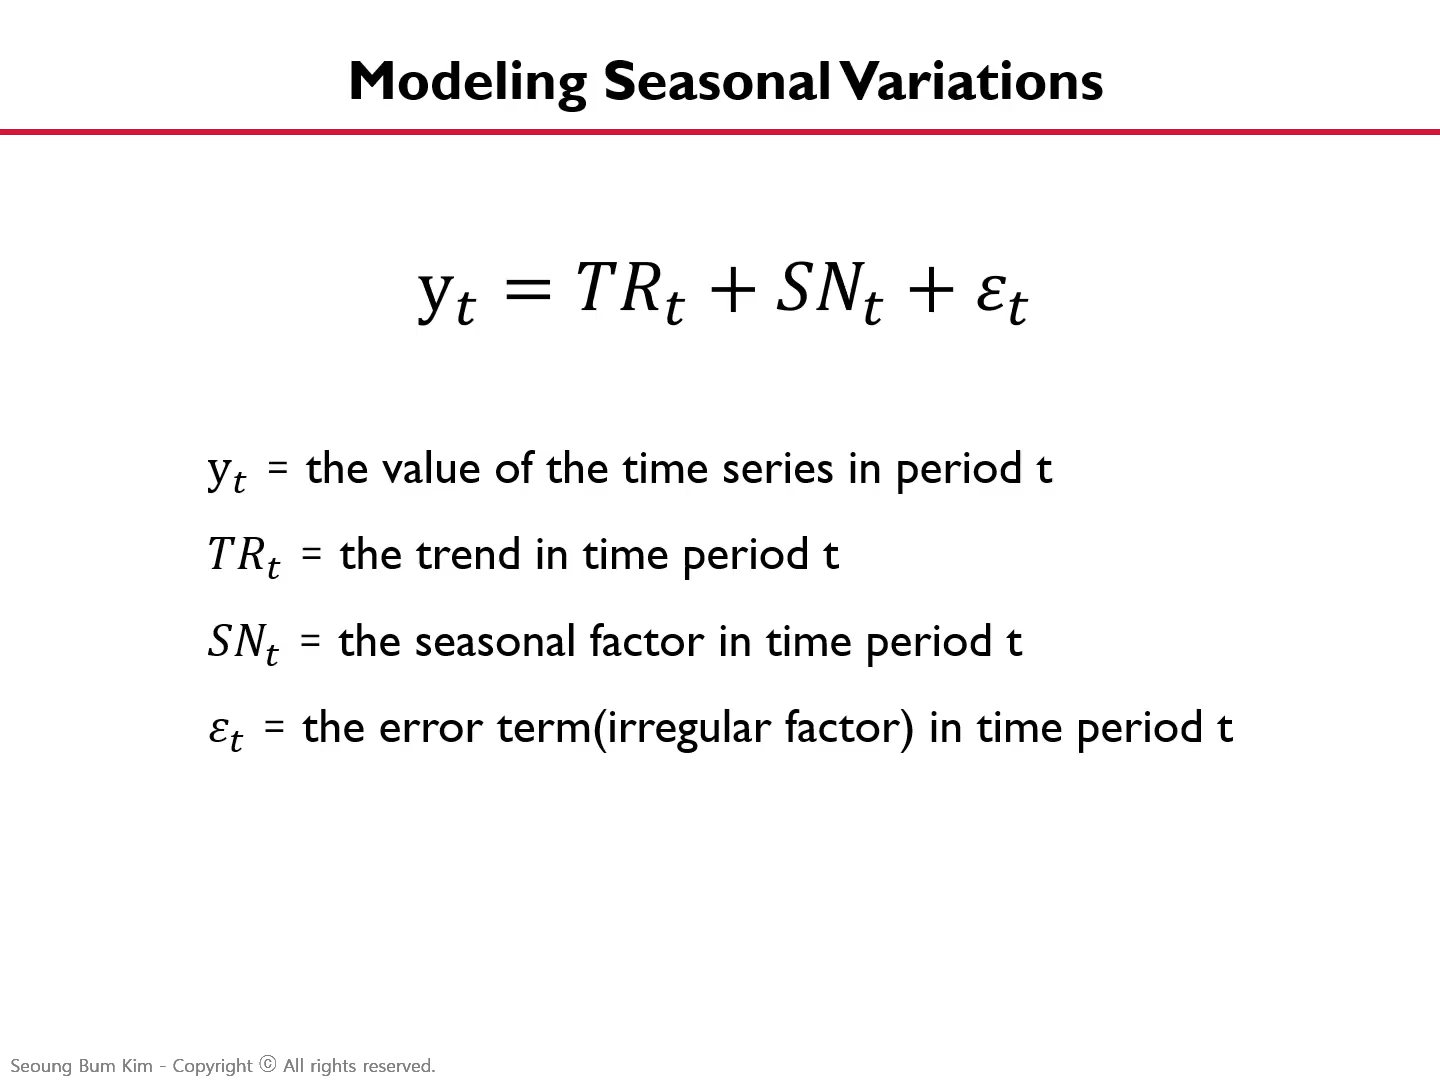
\includegraphics[width=.5\textwidth]{model_0}
\end{center}

이번 정리부터는 유튜브 캡쳐를 나열한 후 정리하려고 하고, 너무 많은 내용을 적기보다는 강의 내용 자체에만 충실하게 적어보려고 한다.

%%
\section{Binary Variable Models}
\begin{center}
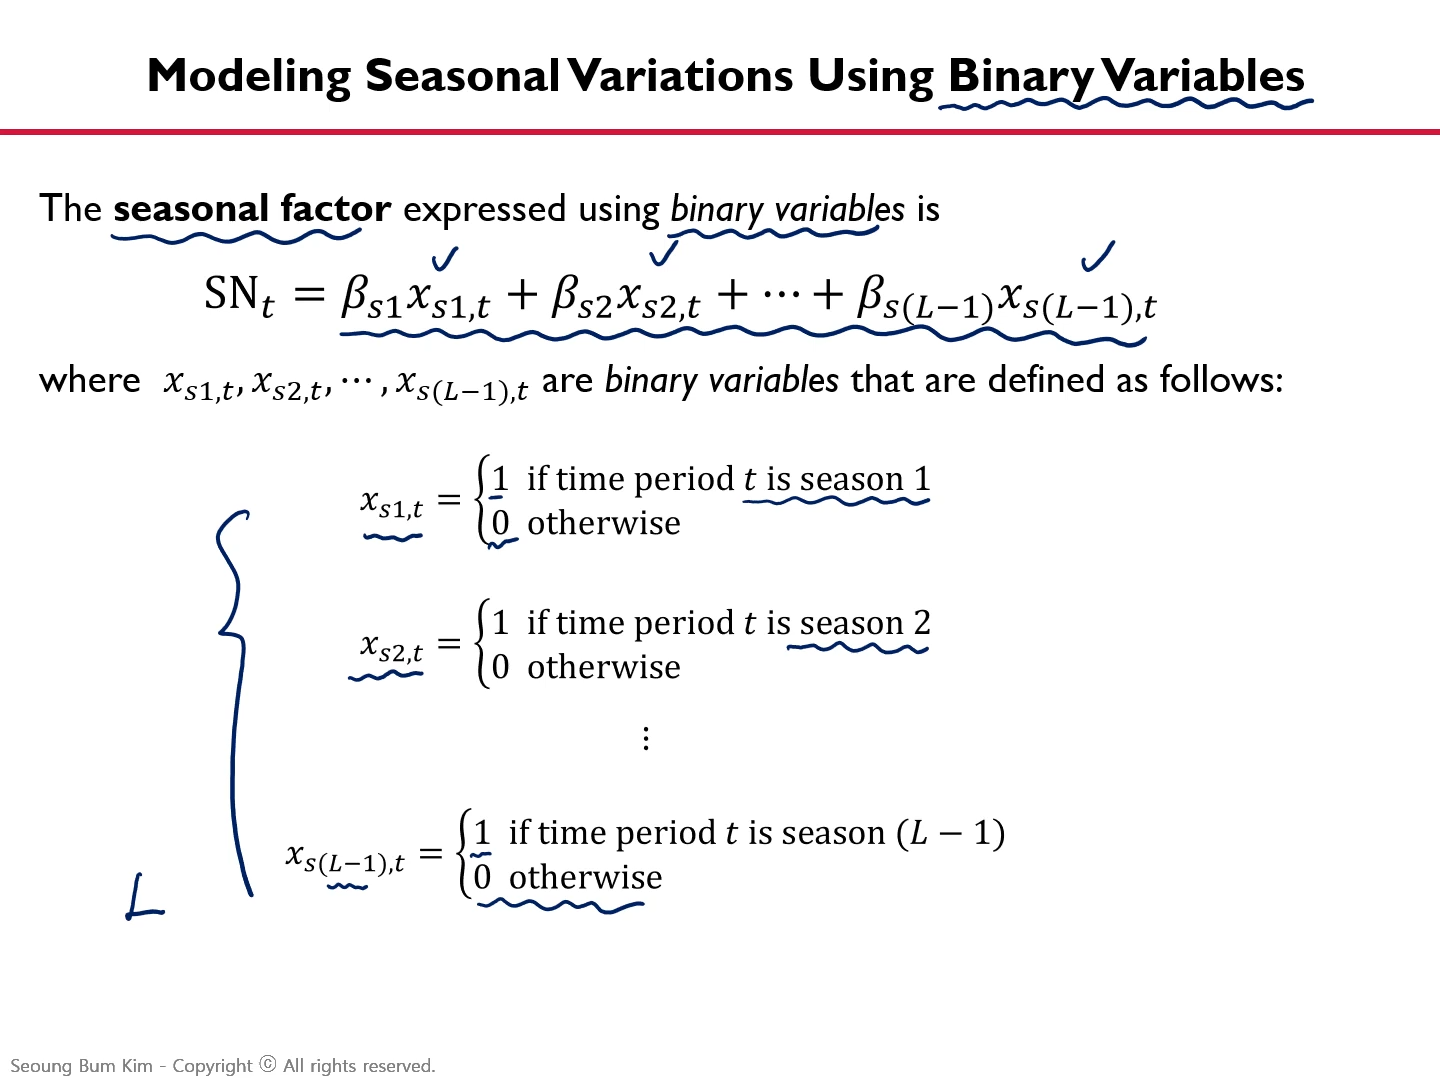
\includegraphics[width=.45\textwidth]{model_1-1}
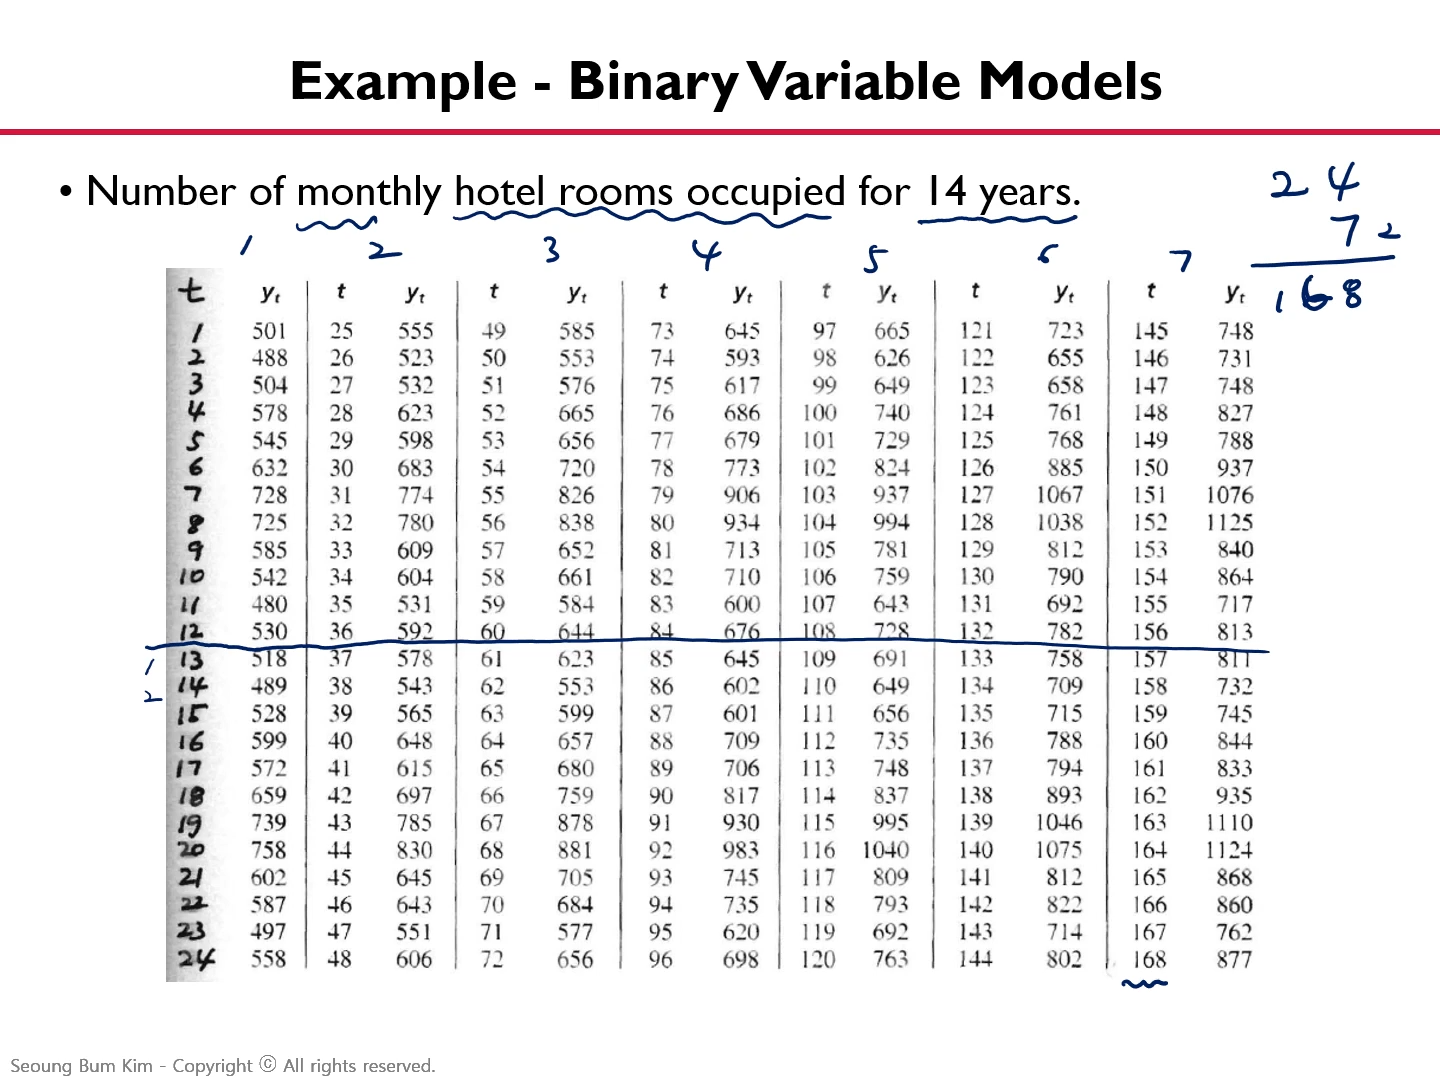
\includegraphics[width=.45\textwidth]{model_1-2}
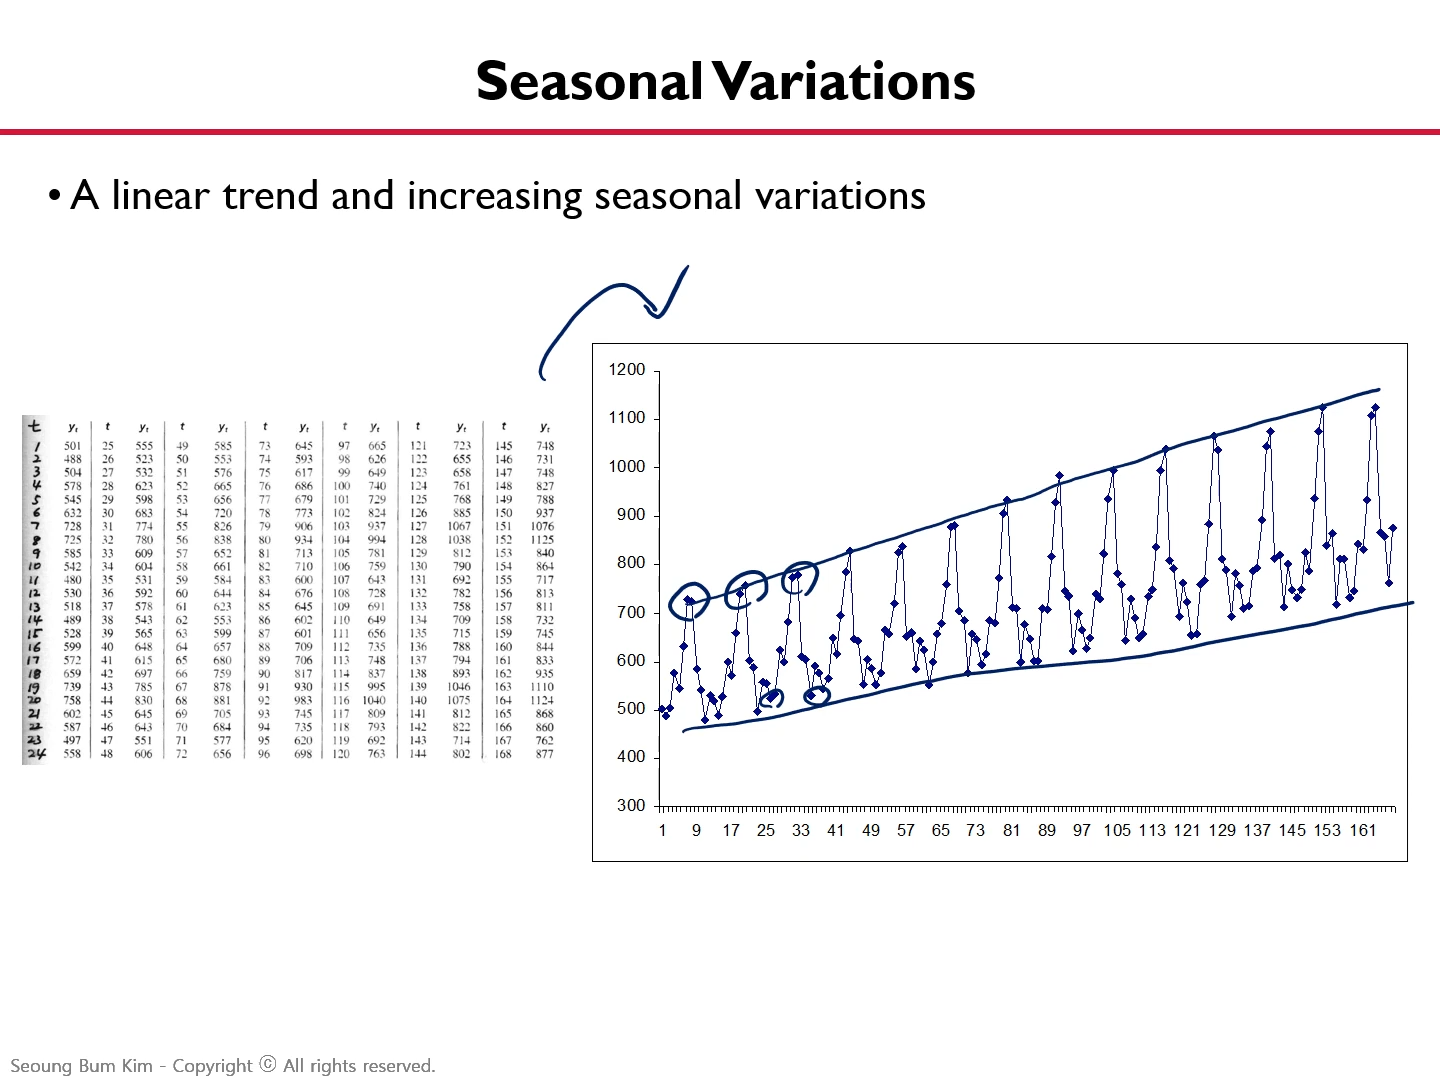
\includegraphics[width=.45\textwidth]{model_1-3}
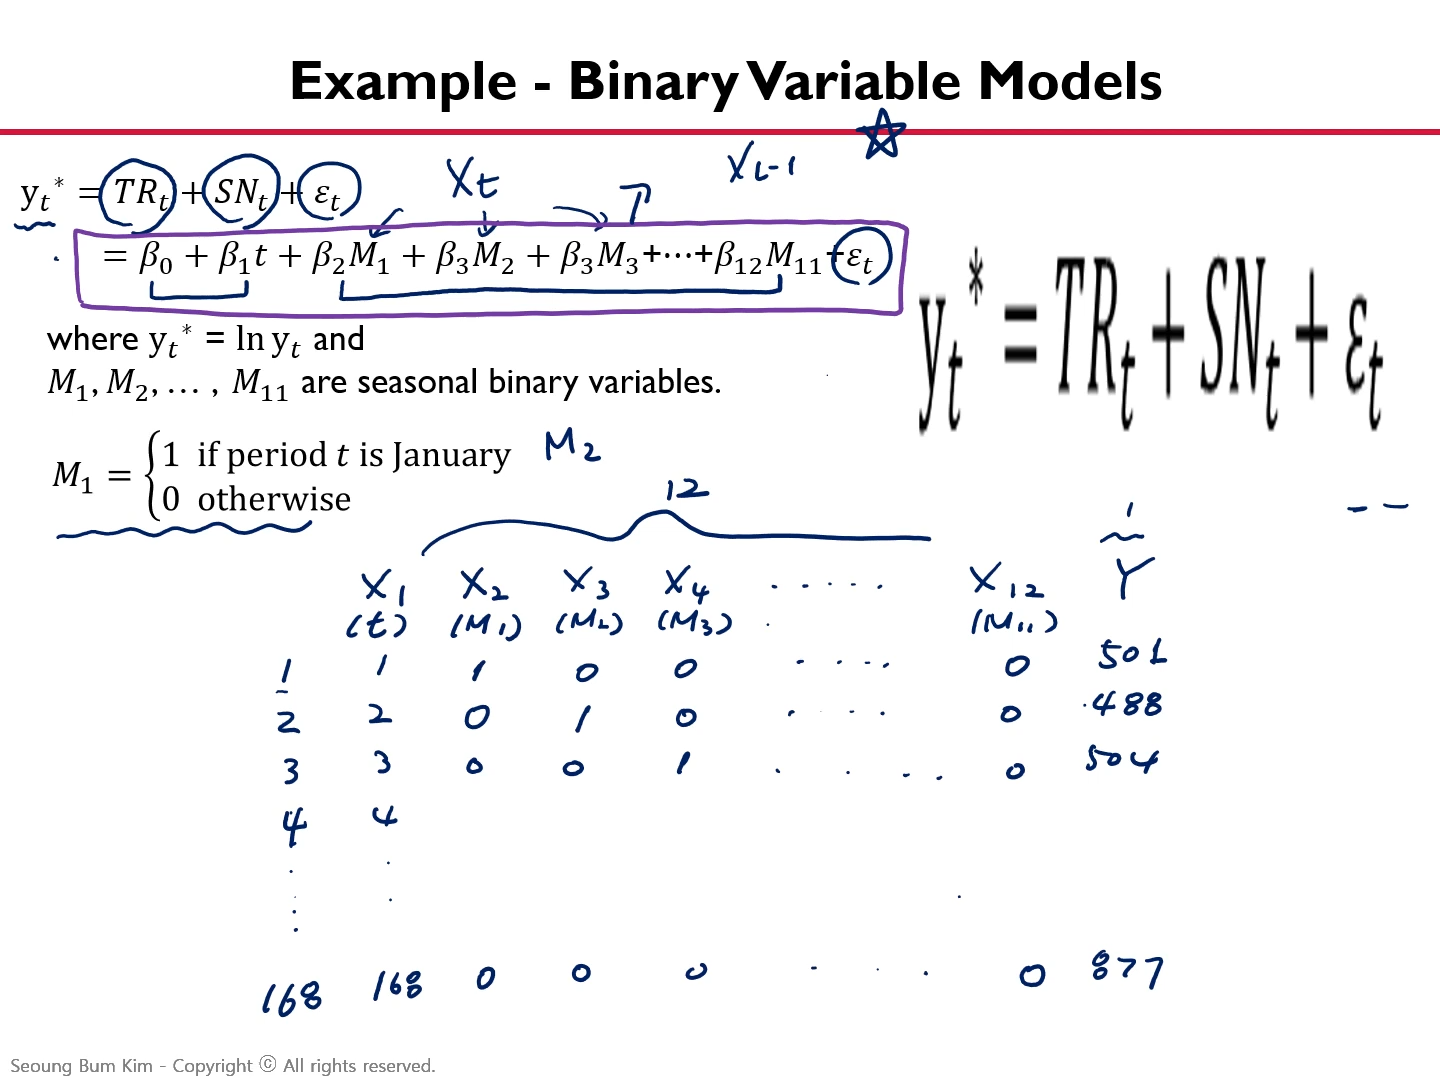
\includegraphics[width=.45\textwidth]{model_1-4}
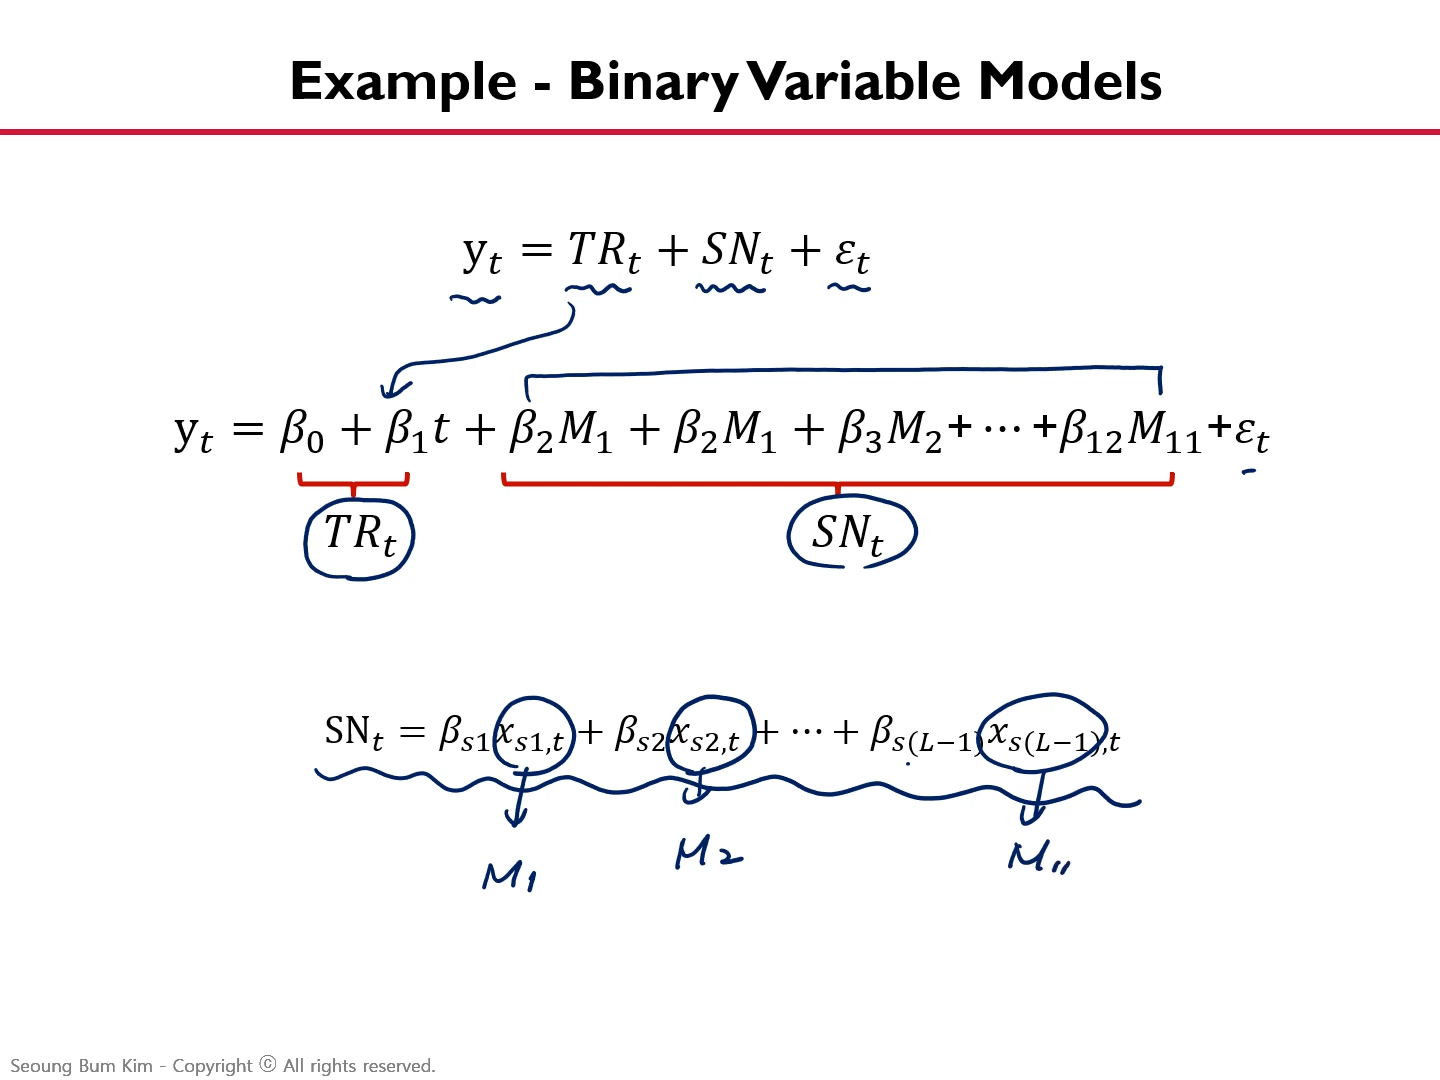
\includegraphics[width=.45\textwidth]{model_1-5}
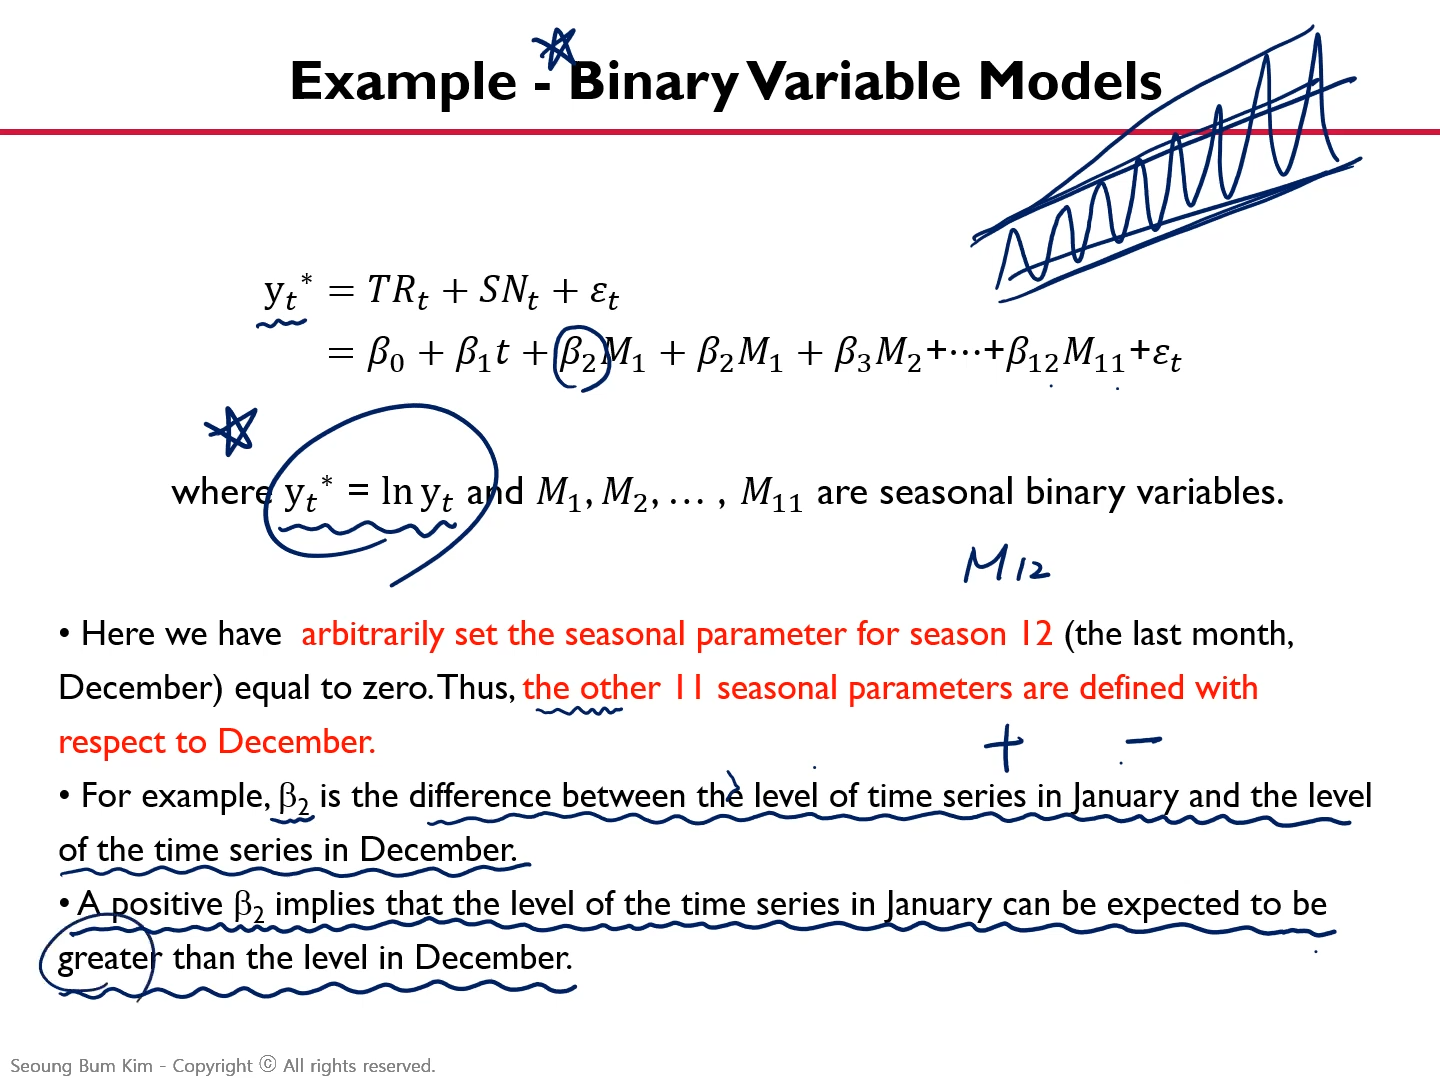
\includegraphics[width=.45\textwidth]{model_1-6}
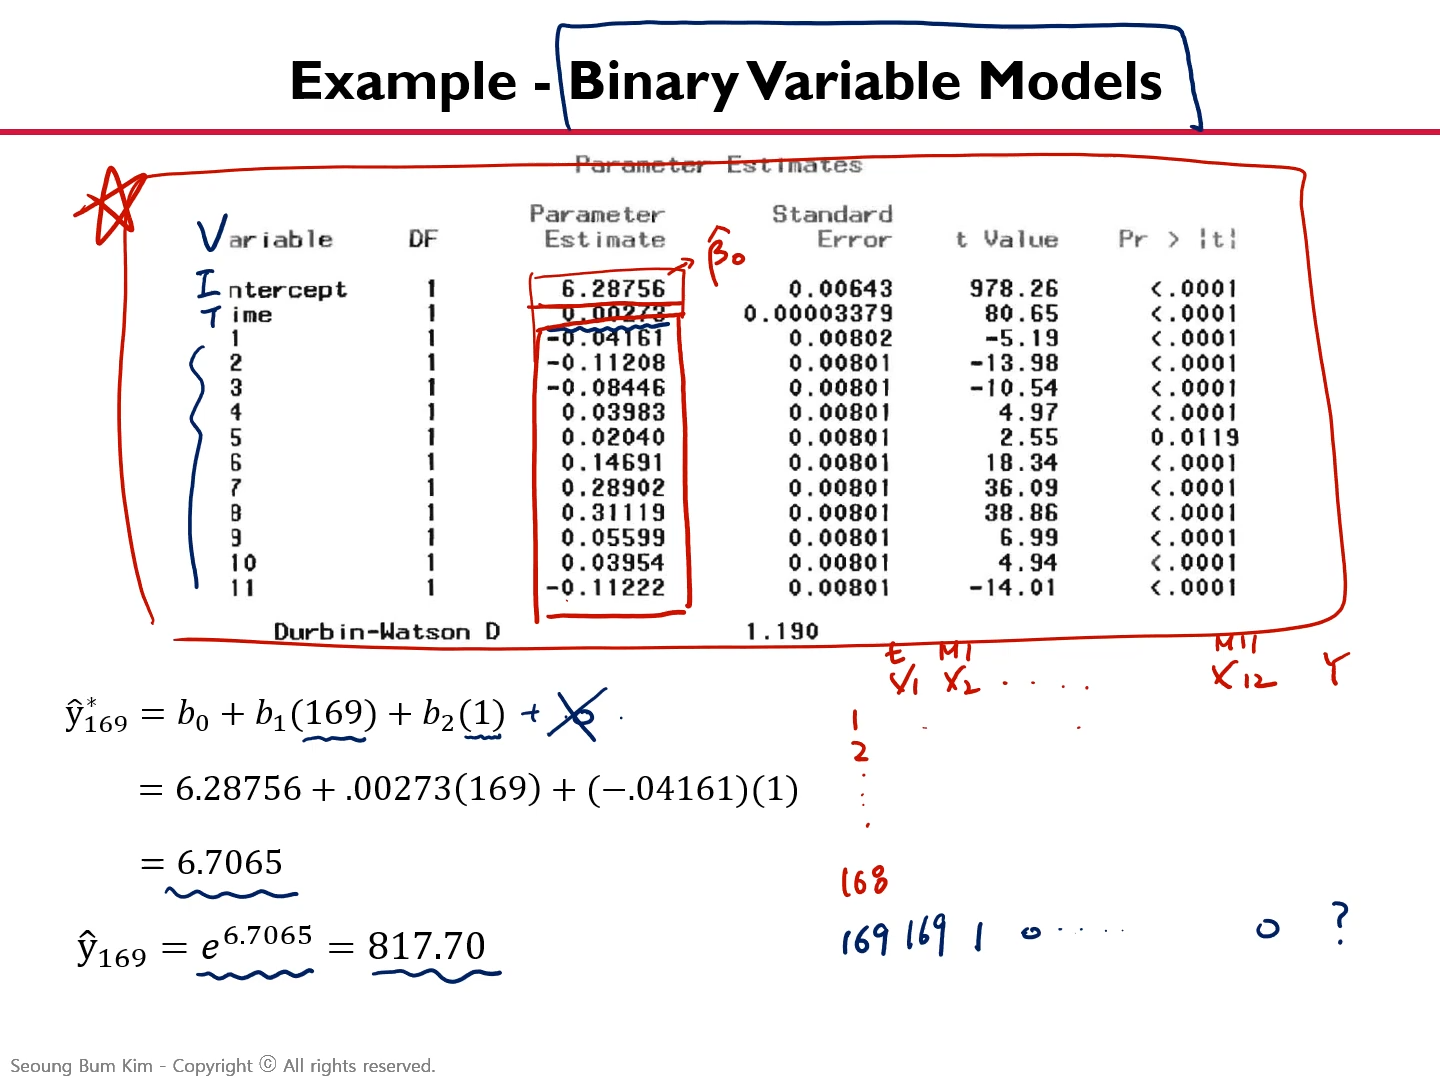
\includegraphics[width=.45\textwidth]{model_1-7}
\end{center}

seasonal variation을 다루기 위한 여러 모델들 중 첫번째로 다루는 모델은 binary variable model이다.
예시로 주어지고 있는 데이터셋은 한 호텔의 투숙된 객실 수에 대한 데이터이다.
시간 \(t\)의 단위는 `월'로 주어져있고, 총 7년의 데이터가 있으므로 \(t\in\{1, 2,\cdots,168\}\)이다.
종속변수는 \(y\)이고 독립변수는 \(x\)이지만, \(x_t=t\)라는 점에서 독립변수를 그냥 \(t\)라고 봐도 될 것 같다.
다시 말해서, 몇 번째 달(\(t\))에 몇 개의 객실들(\(y\))이 투숙되어 있는지 하는 단변수 회귀 (univariate regression) 문제이다.

이전 강의의 예에서는 추세(trend, $TR_t$)만을 예측모델로 잡았었다. 하지만, 세 번째 슬라이드에서 보듯 계절성이 뚜렷이 드러나고 있으므로, 예측모델 \(f_\beta\)을 설정할 때 추세 말고도 계절성(seasonal variation, $SN_t$)도 고려할 것이다.
즉
\begin{equation}\label{model_1-1}
f_\beta(t) = TR_t+SN_t
\end{equation}
이고
\[y_t=f_\beta(t)+\epsilon_t\]
이다.
추세는 일차함수(affine function)로 표현할 것이어서
\[TR_t = \beta_0+\beta_1 t\]
이고, 계절성은 각각의 계절에 대하여 상수회귀(no trend, constant regression)로 둔다.
식으로 표현하면
\[SN_t = \begin{cases}
\beta_2&(t=12n+1)\\
\beta_3&(t=12n+2)\\
&\vdots\\
\beta_{11}&(t=12n+10)\\
0&(t=12n+11)\\
\end{cases}\qquad\qquad(\text{단, \(n=0,1,2,\cdots,6)\)}\]
이다.
이것을 표현하기 위해서 강의에서는 \(M_1\), \(M_2\), \(\cdots\), \(M_{11}\)을 사용하고 있는데, 이건 각 월에 대한 characteristic function (indicator function)으로 이해하면 될 것 같다.
여하튼, 식 \eqref{model_1-1}을 다시 정리하면
\begin{equation}\label{model_1-2}
f_\beta(t) = \begin{cases}
\beta_0+\beta_2+\beta_1t&(t=12n+1)\\
\beta_0+\beta_3+\beta_1t&(t=12n+2)\\
&\vdots\\
\beta_0+\beta_{11}+\beta_1t&(t=12n+10)\\
\beta_0+\beta_1t&(t=12n+11)\\
\end{cases}\qquad\qquad(\text{단, \(n=0,1,2,\cdots,6)\)}
\end{equation}
이 된다.
%\(M_{12}\)는 굳이 사용하지 않았다.
각 월(1월 \(\sim\) 11월)에 대한 정보를 담고 있는 항은 \(\beta_2\), \(\cdots\), \(\beta_{11}\)이다.
그리고 12월에 대한 정보를 담고 있는 항은 없다.
하지만 문제가 되지 않는다.

다시 말해서, 1월부터 11월까지의 월들에 각각 어떤 기본값을 부여할 지에 대해서는 매개변수 \(\beta_2\), \(\cdots\), \(\beta_{11}\)로 조정하면 된다.
하지만, \(y\)절편에 해당하는 \(\beta_0\)를 이미 설정해놓았으므로, 12월에는 \(\beta_0\)라는 기본값을 부여받게 되는 것이다.
12월에 대한 정보는 \(\beta_0\)를 통해 조정될 수 있는 것이다.
새로운 매개변수 \(\beta_{12}\)를 도입할 수도 있지만, 굳이 그렇게 하는 게 의미가 없는 것이다.

그런데, 어차피 그렇게 할거면, trend를 설정할 때, \(y\)절편이 없는 일차함수로 잡은 다음 \(M_1\), \(M_2\), \(\cdots\), \(M_{12}\)를 설정해도 같은 의미가 될 것이다.
그렇게 하는 편이 보기에 깔끔해보인다.
하지만, 지금과 같은 방법을 취하는 것이 아마도 통계 방면에서의 관습인 게 아닐까 싶기도 하다.

이렇게 parametric model \(f_\beta\)를 설정했다.
그 다음으로 하는 것은 기존의 회귀분석(ordinary regression analysis)을 진행하는 것이다.
강의에서는 45분 32초쯤에 `일반적인 최소제곱법(LSE, least square estimation ; OLS ordinary least square, ordinary least squares)'을 사용하는 것이다.
표에서 관측치가 주어져있었다.
\begin{align*}
\text{관측치}
&=\{(t,y_t):t=1,2,\cdots,168\}\\
&=\{(1,501), (2,488),\cdots,(168,877)\}
\end{align*}
이걸 가지고 MSE를 계산하면
\[\text{MSE}=\frac1{168}\sum_{t=1}^{168}\left(y_t-f_\beta(t)\right)^2\]
이 된다.
\(MSE\)를 \(\beta_0\), \(\beta_1\), \(\cdots\), \(\beta_{11}\)로 편미분한 것을 0으로 두면 미지수가 12개이고 식이 12개인 연립방정식이 나오는데, 그 연립방정식을 풀어 근을 \(\beta_0=\hat\beta_0\), \(\beta_1=\hat\beta_1\), \(\cdots\), \(\beta_{11}=\hat\beta_{11}\) 들을 가지고 최적의 함수 \(\hat f\)를 찾을 수 있다.

이 계산들은 보통은 컴퓨터를 통해, 몇개의 명령어를 입력하여 계산하는 것 같고, 마지막 캡쳐의 표에 이 \(\hat\beta_i\)들의 값이 적혀있는 것으로 보인다.

%%
\section{Trigonometric Models}
\begin{center}
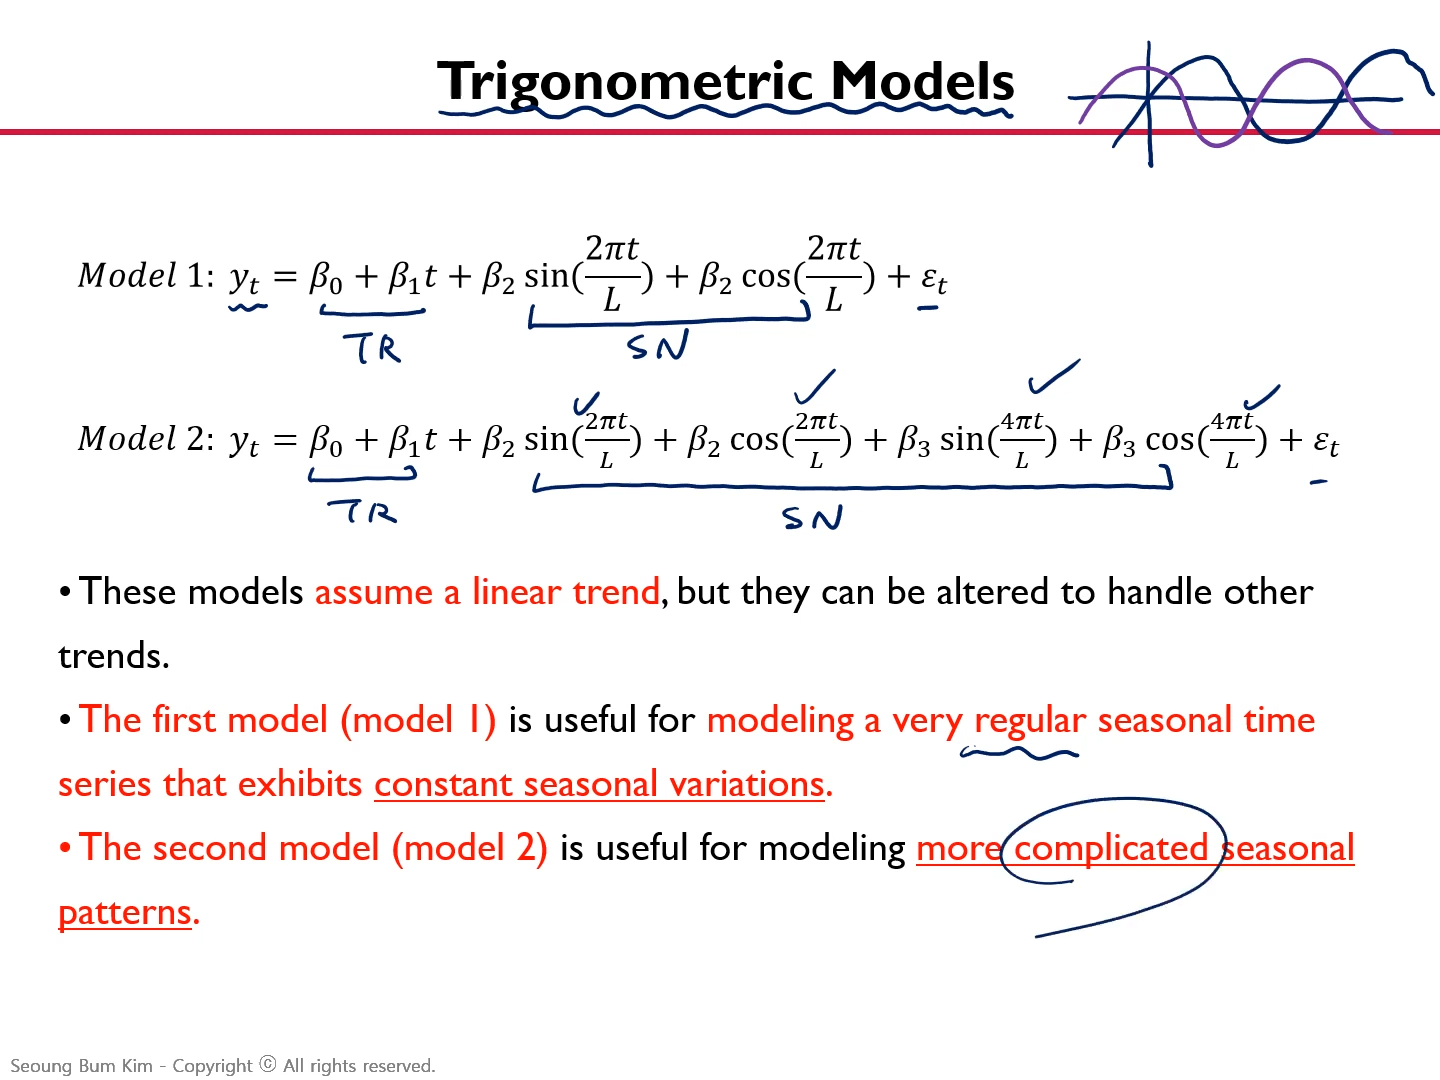
\includegraphics[width=.45\textwidth]{model_2-1}
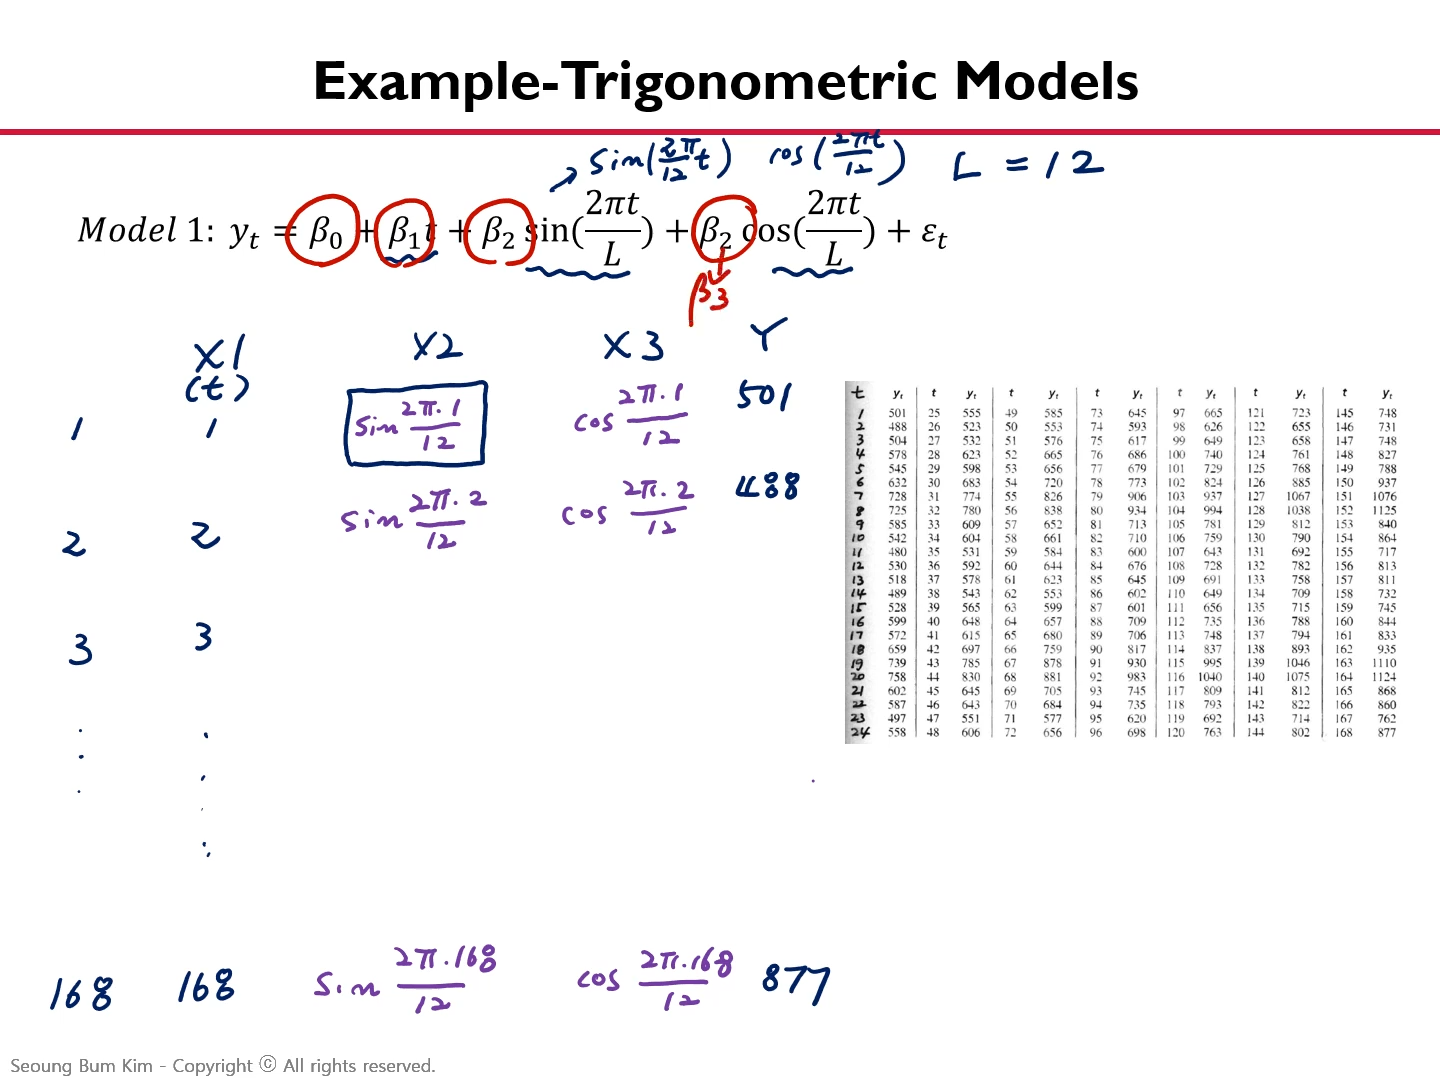
\includegraphics[width=.45\textwidth]{model_2-2}
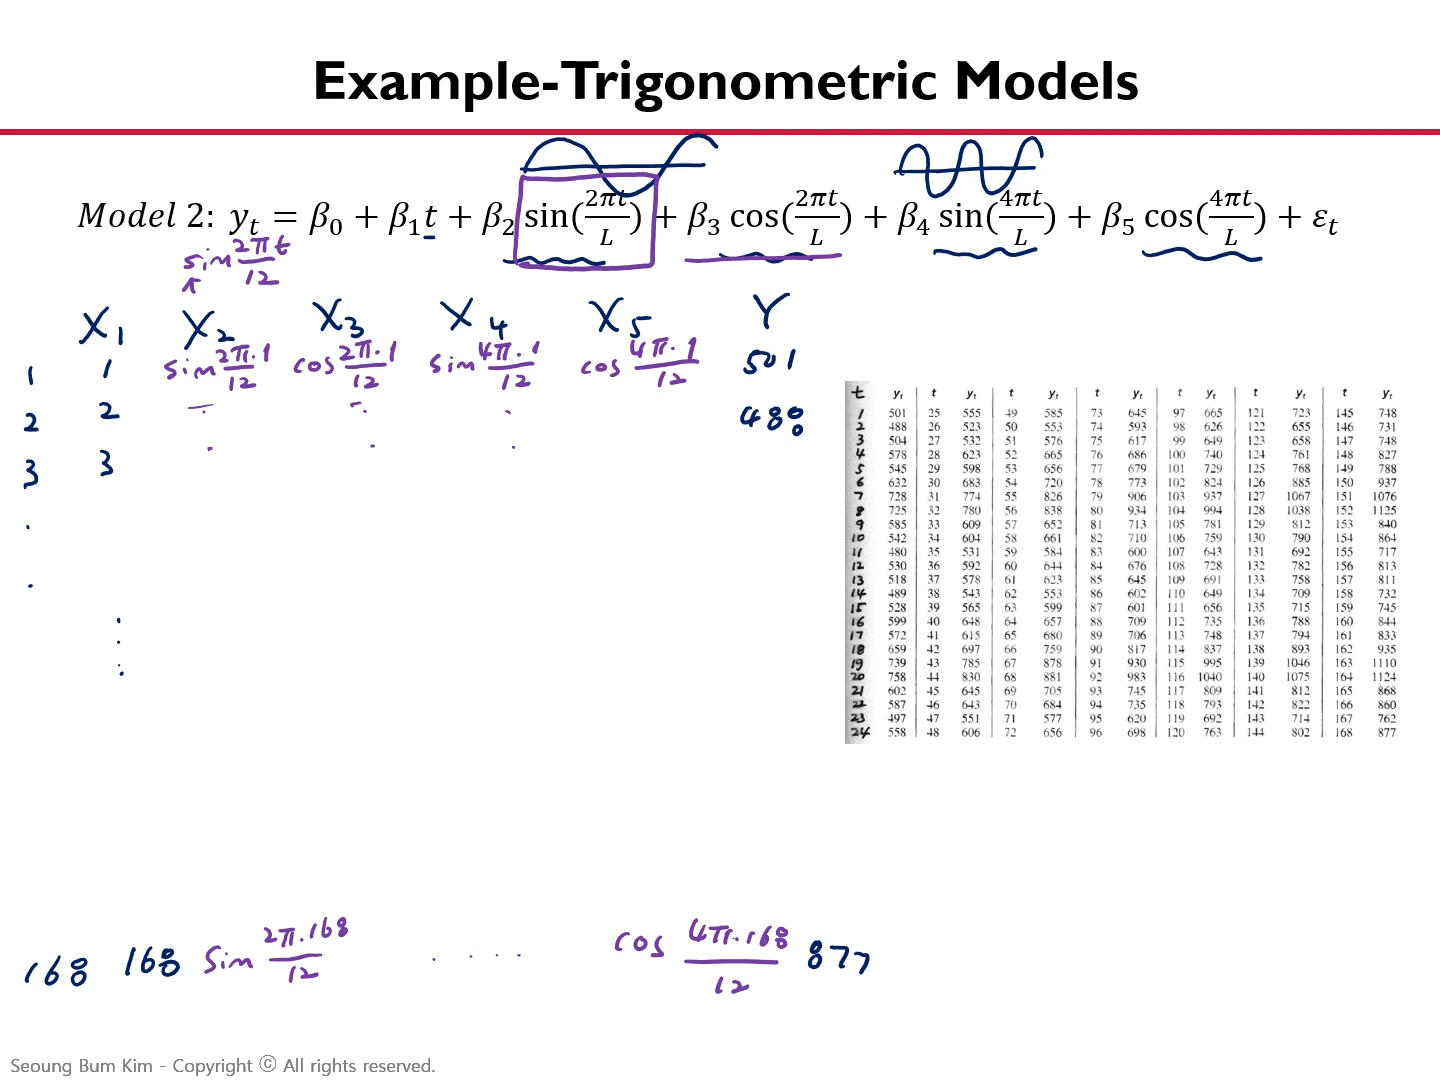
\includegraphics[width=.45\textwidth]{model_2-3}
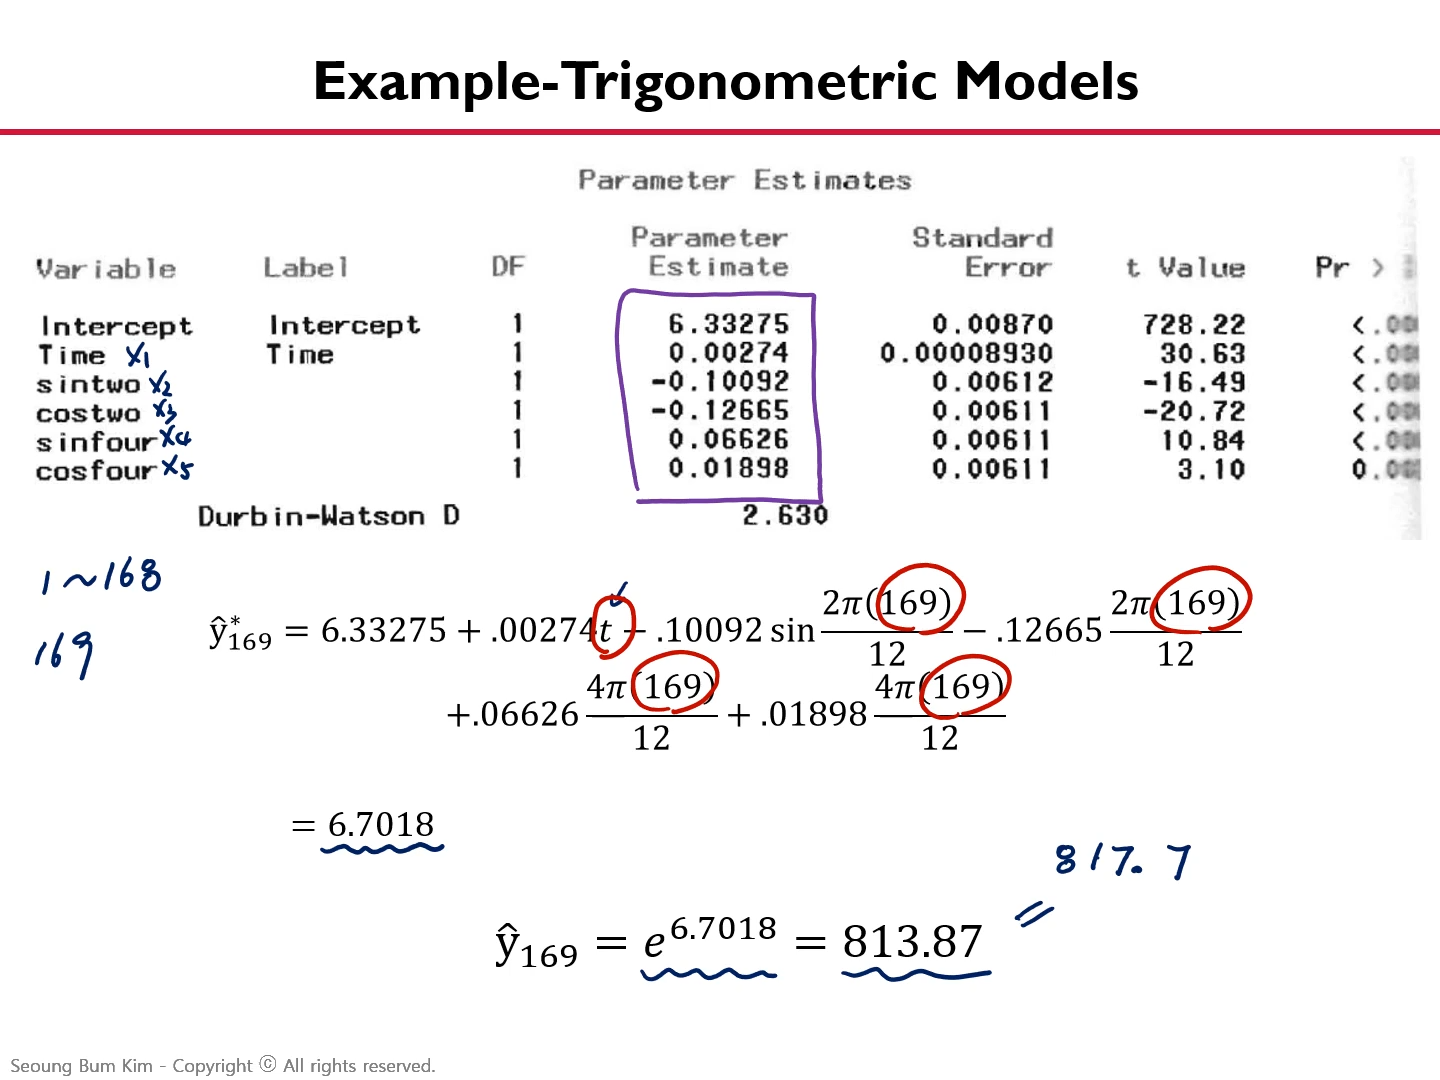
\includegraphics[width=.45\textwidth]{model_2-4}
\end{center}

%%
\section{Growth Curve Models}
\begin{center}
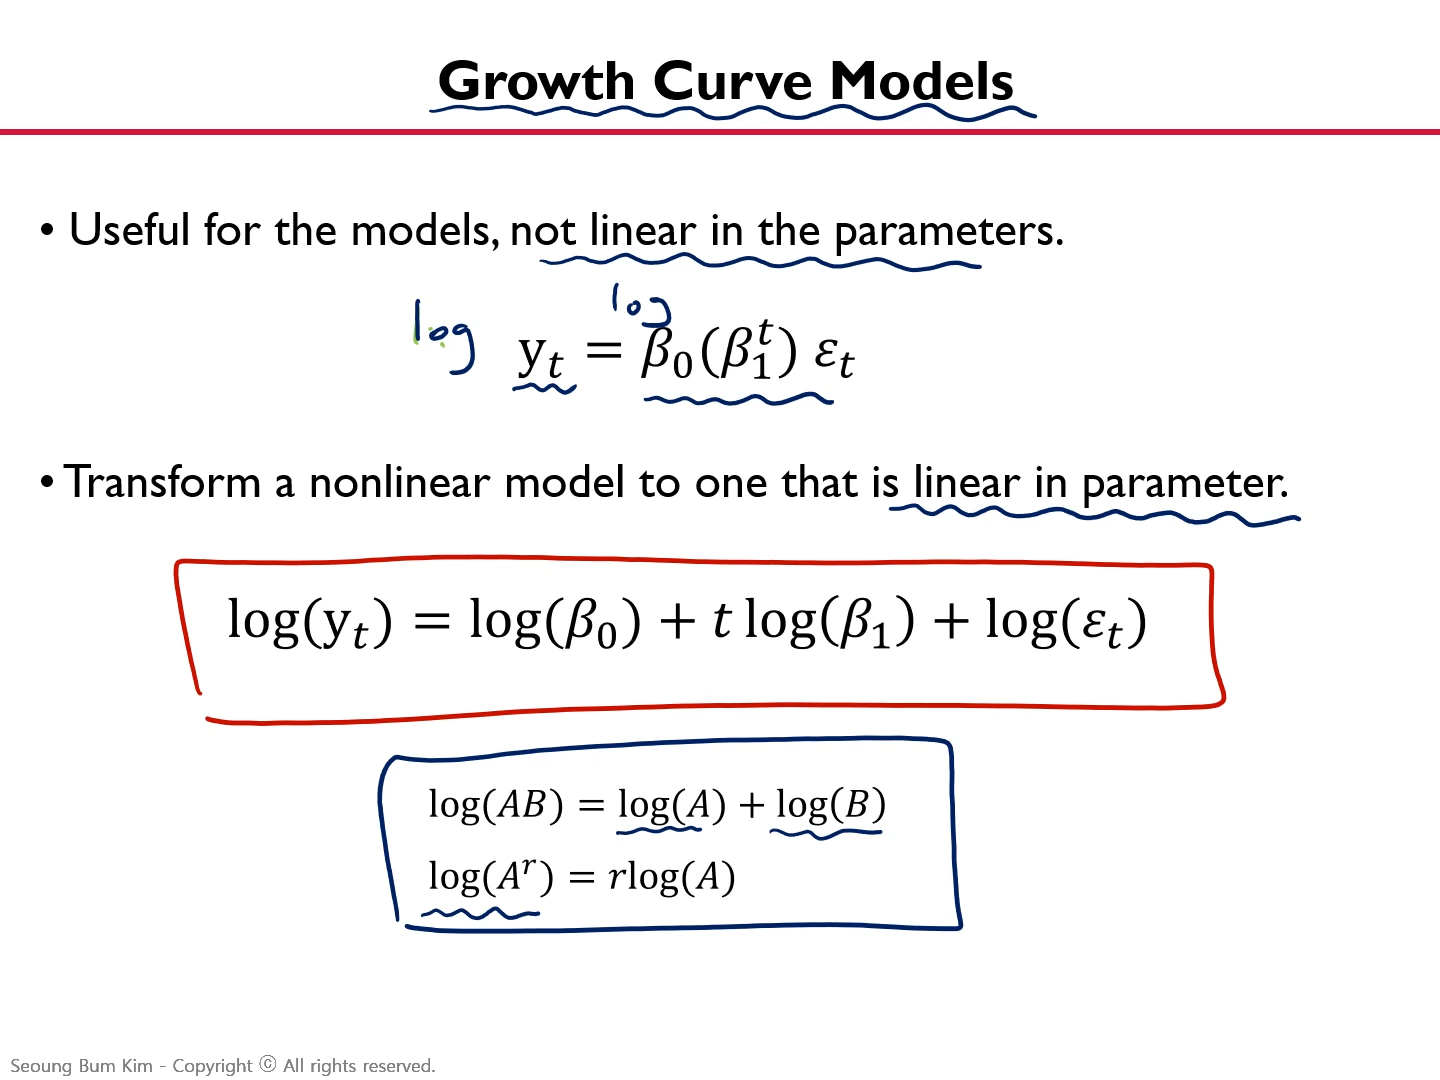
\includegraphics[width=.45\textwidth]{model_3-1}
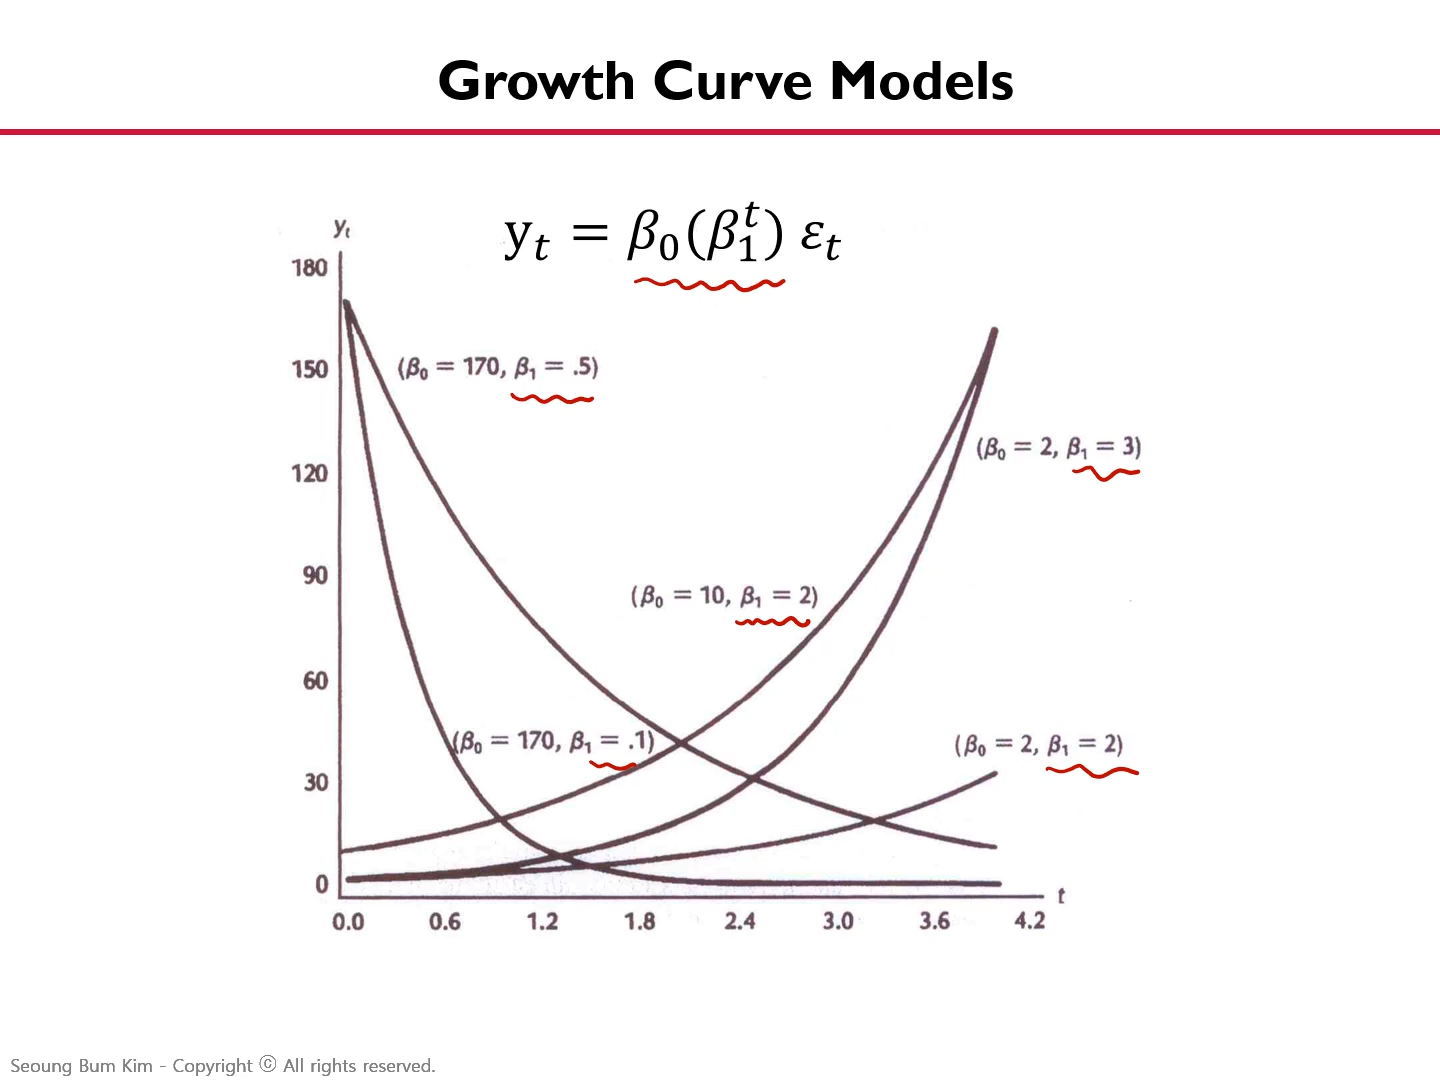
\includegraphics[width=.45\textwidth]{model_3-2}
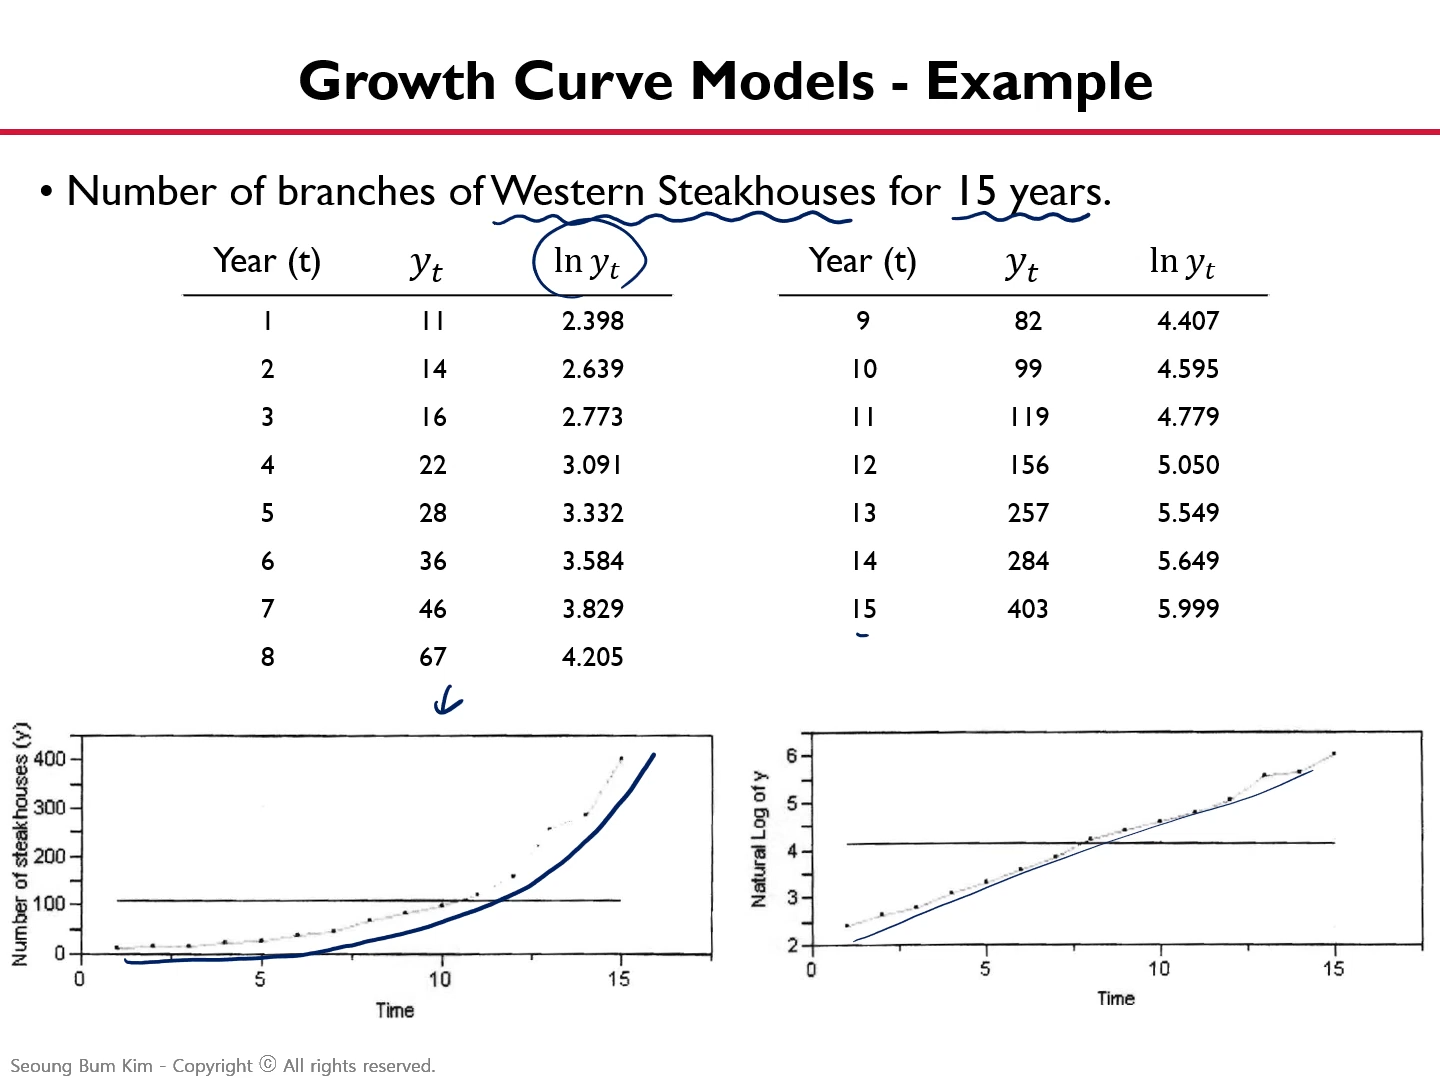
\includegraphics[width=.45\textwidth]{model_3-3}
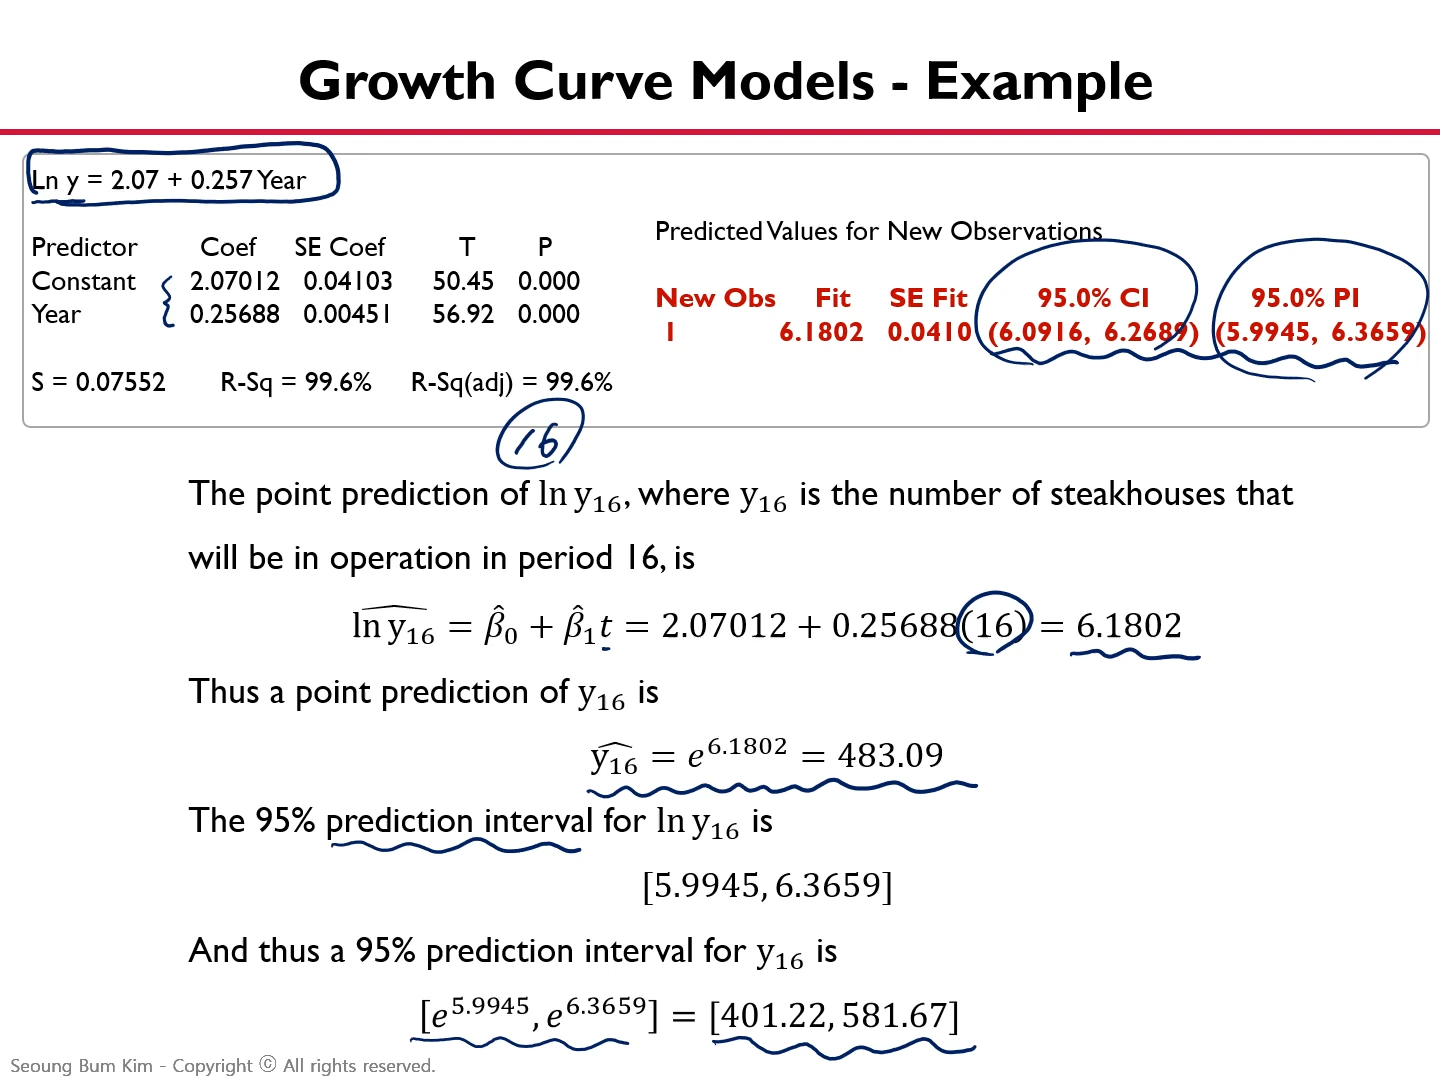
\includegraphics[width=.45\textwidth]{model_3-4}
\end{center}

%%
\section{First-Order Autoregressive Process}
\begin{center}
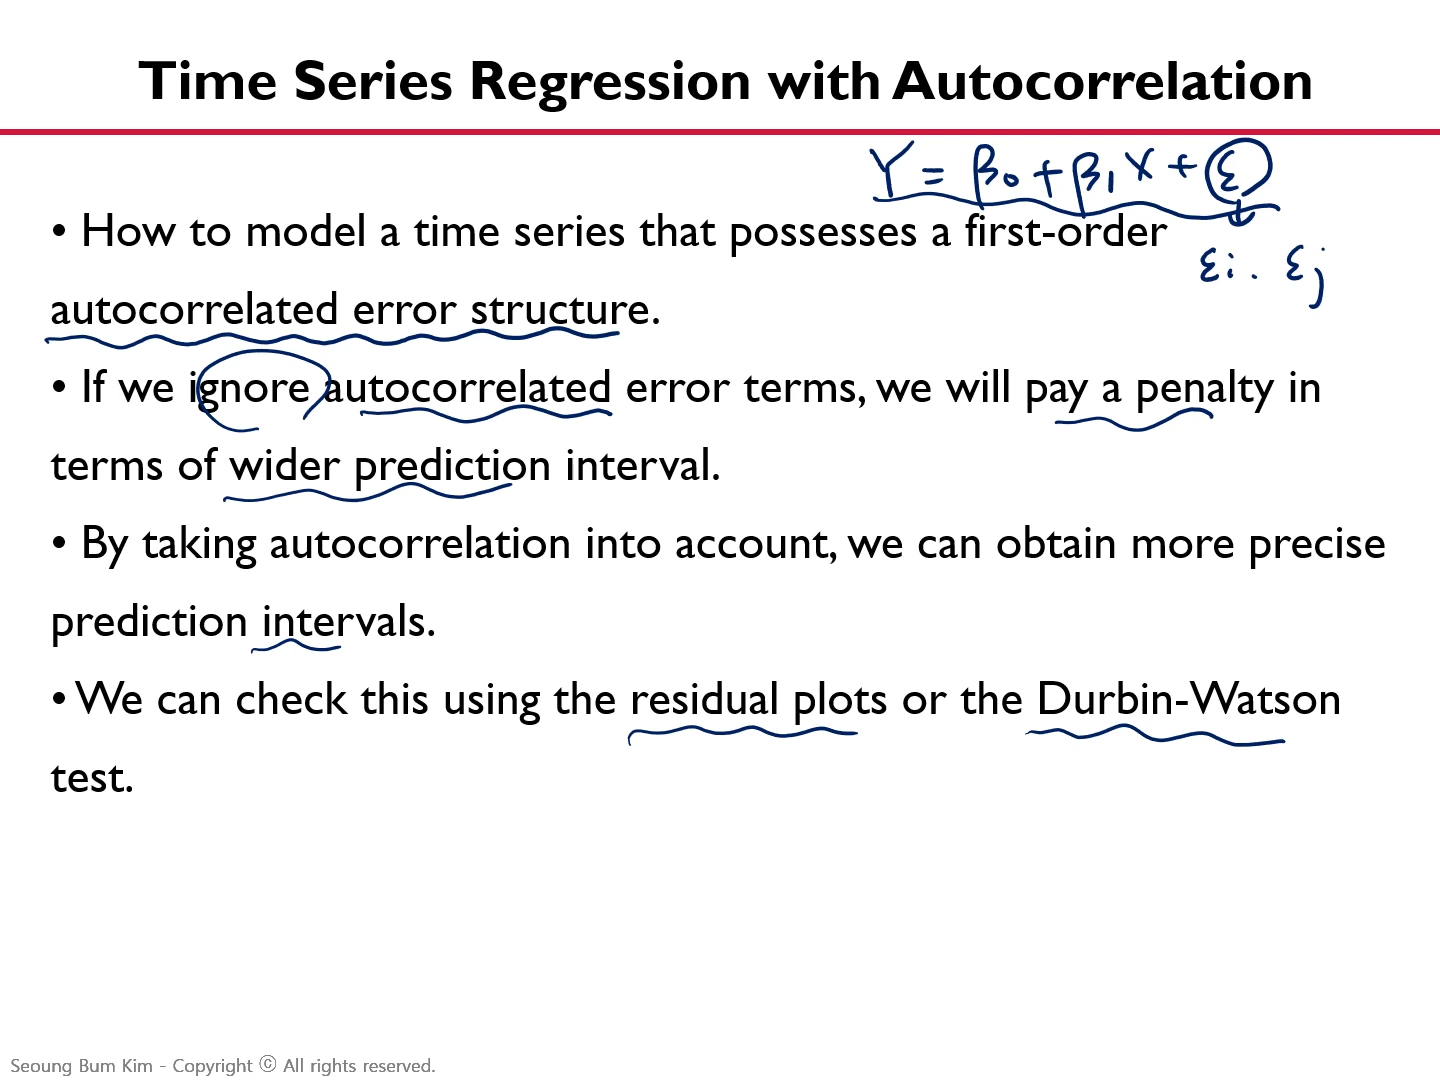
\includegraphics[width=.45\textwidth]{model_4-1}
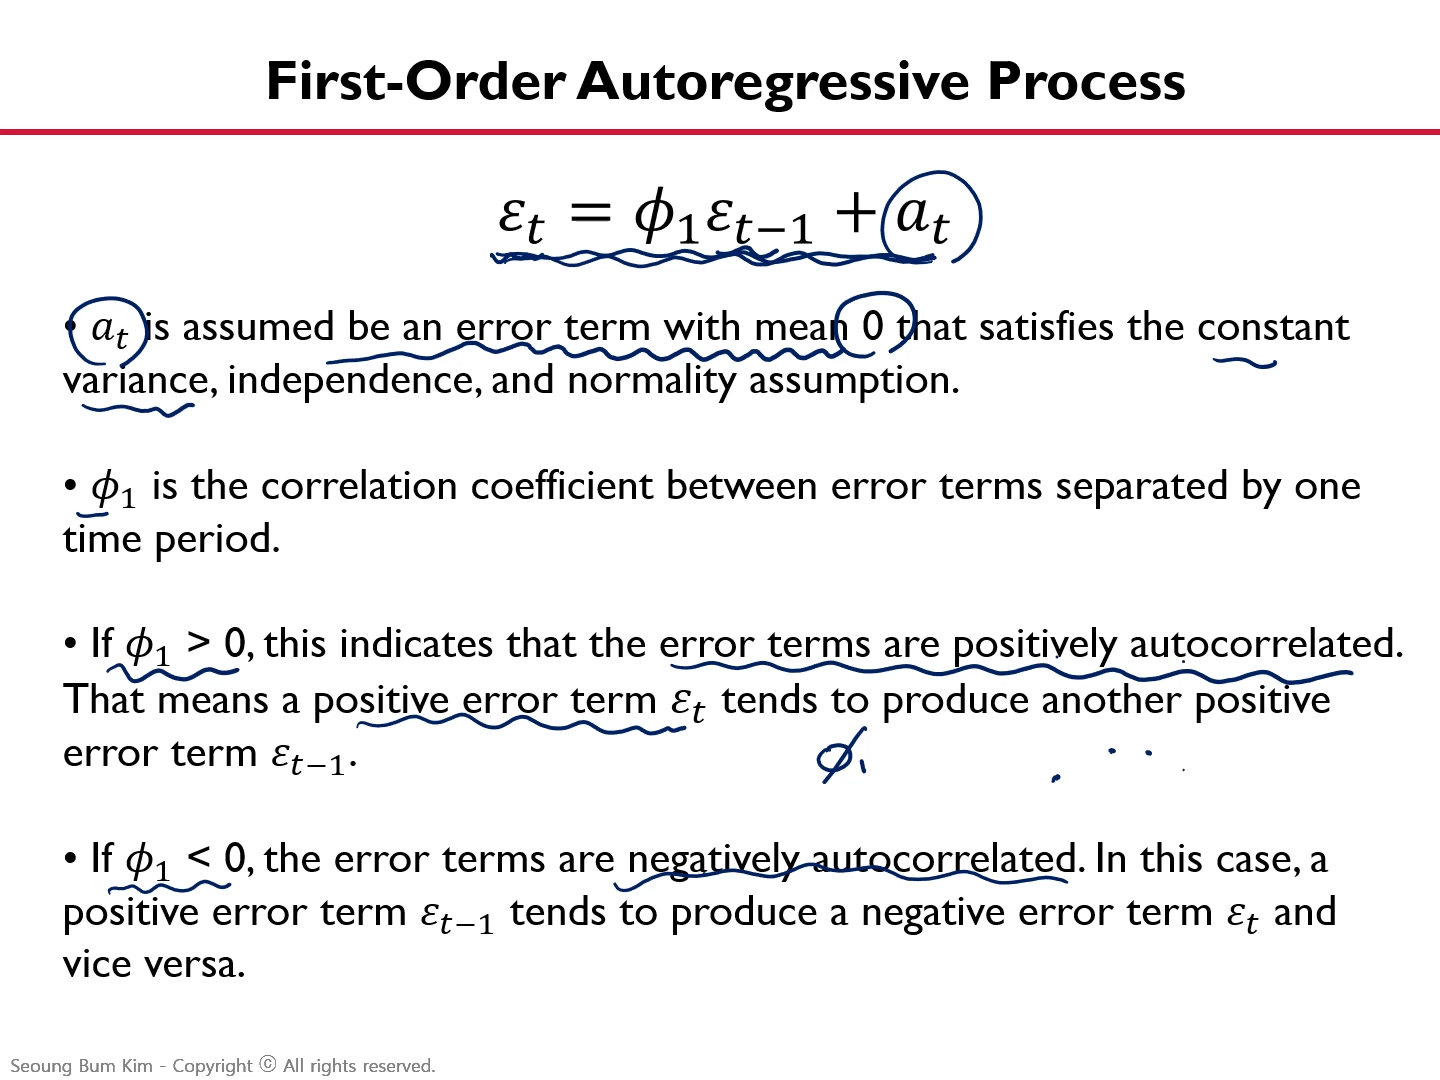
\includegraphics[width=.45\textwidth]{model_4-2}
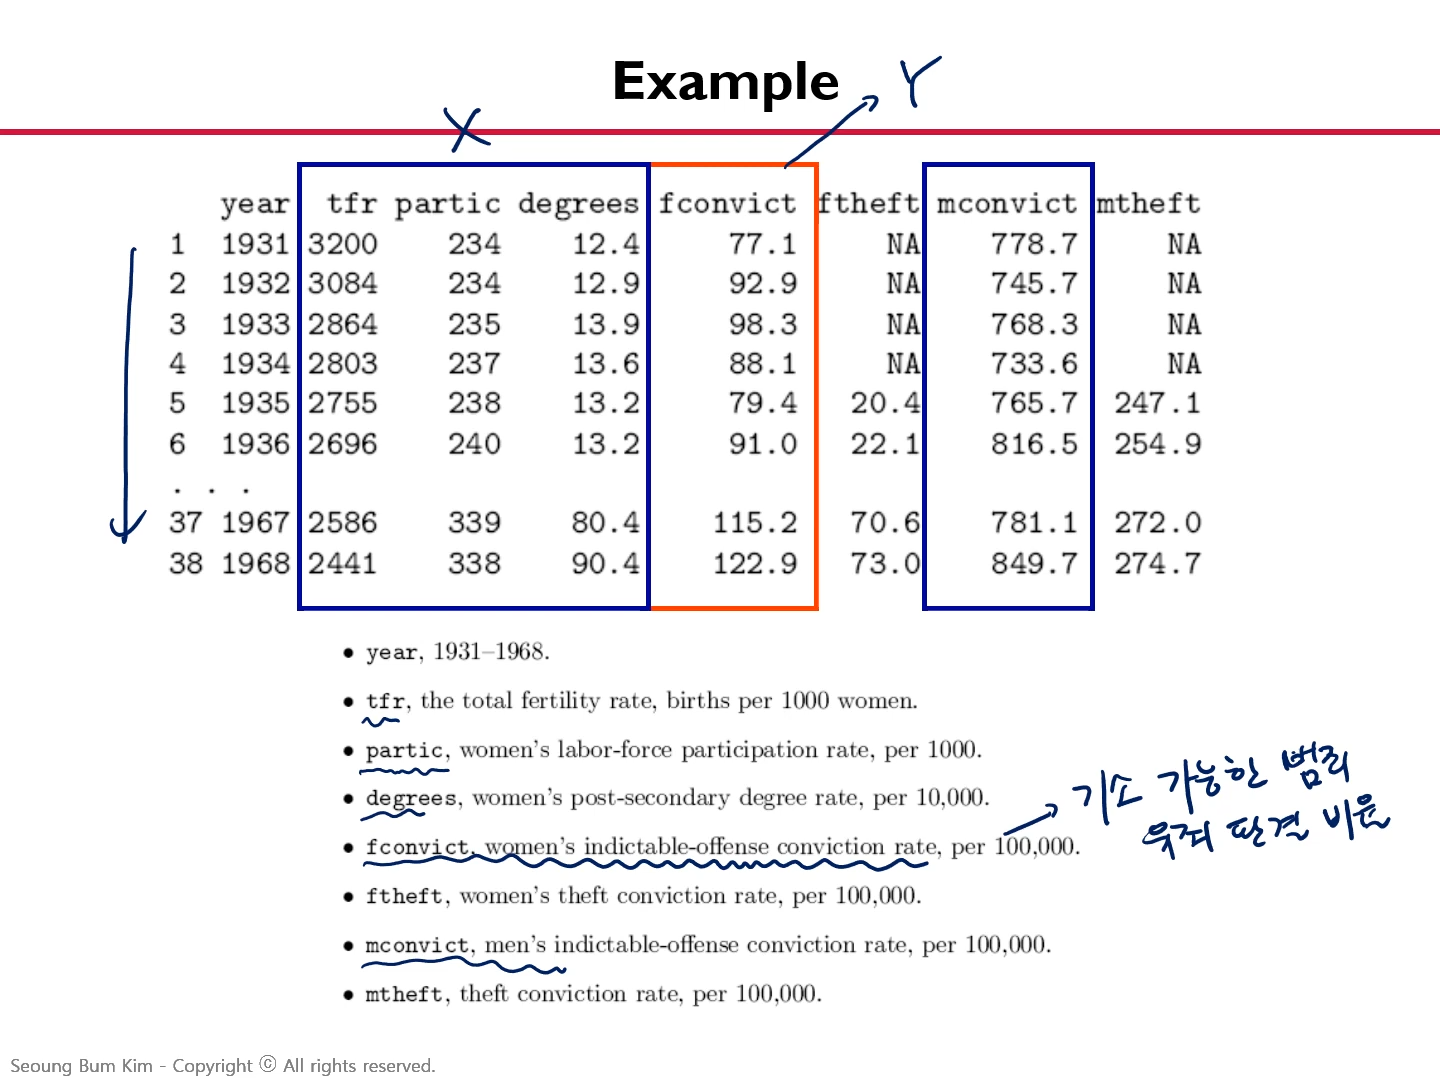
\includegraphics[width=.45\textwidth]{model_4-3}
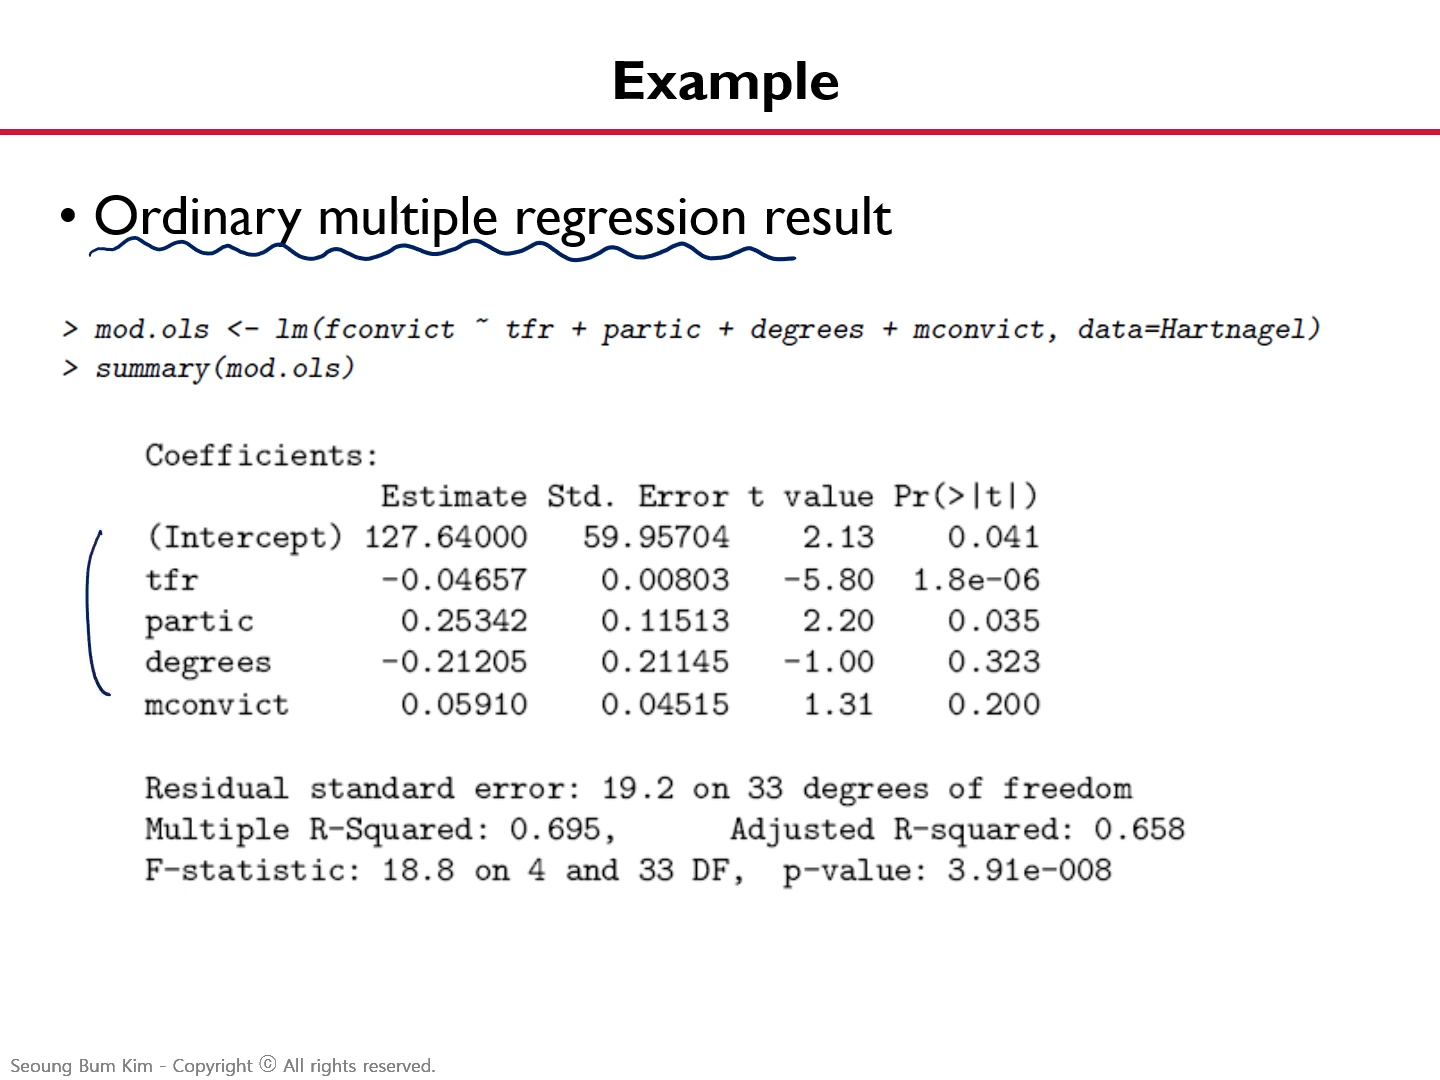
\includegraphics[width=.45\textwidth]{model_4-4}
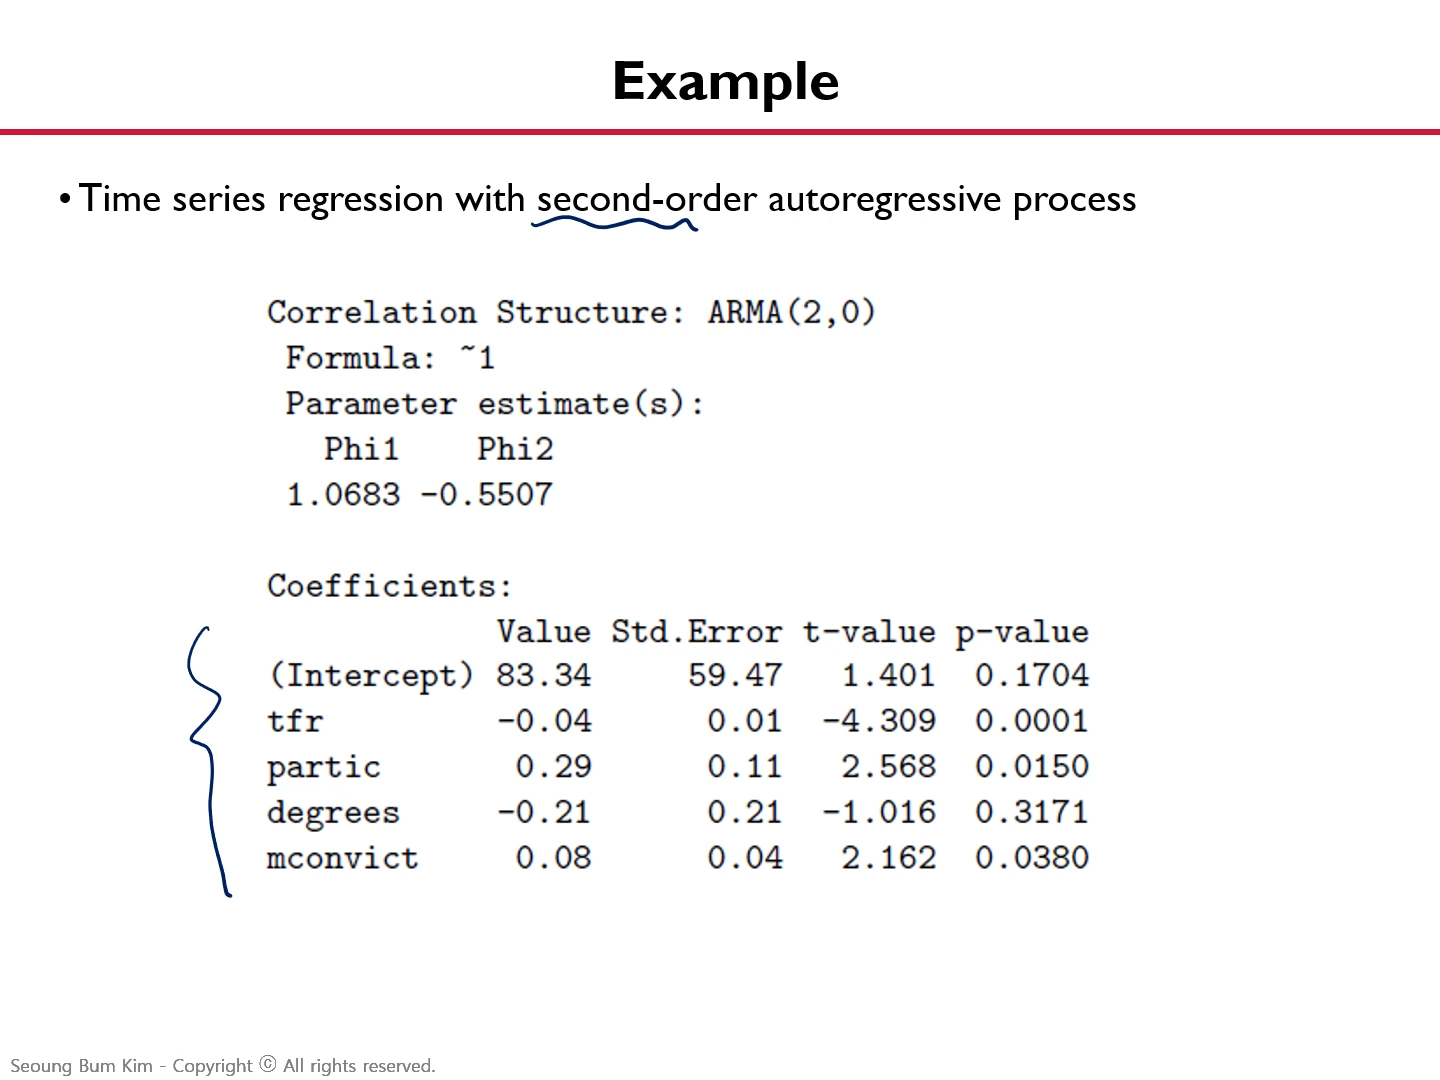
\includegraphics[width=.45\textwidth]{model_4-5}
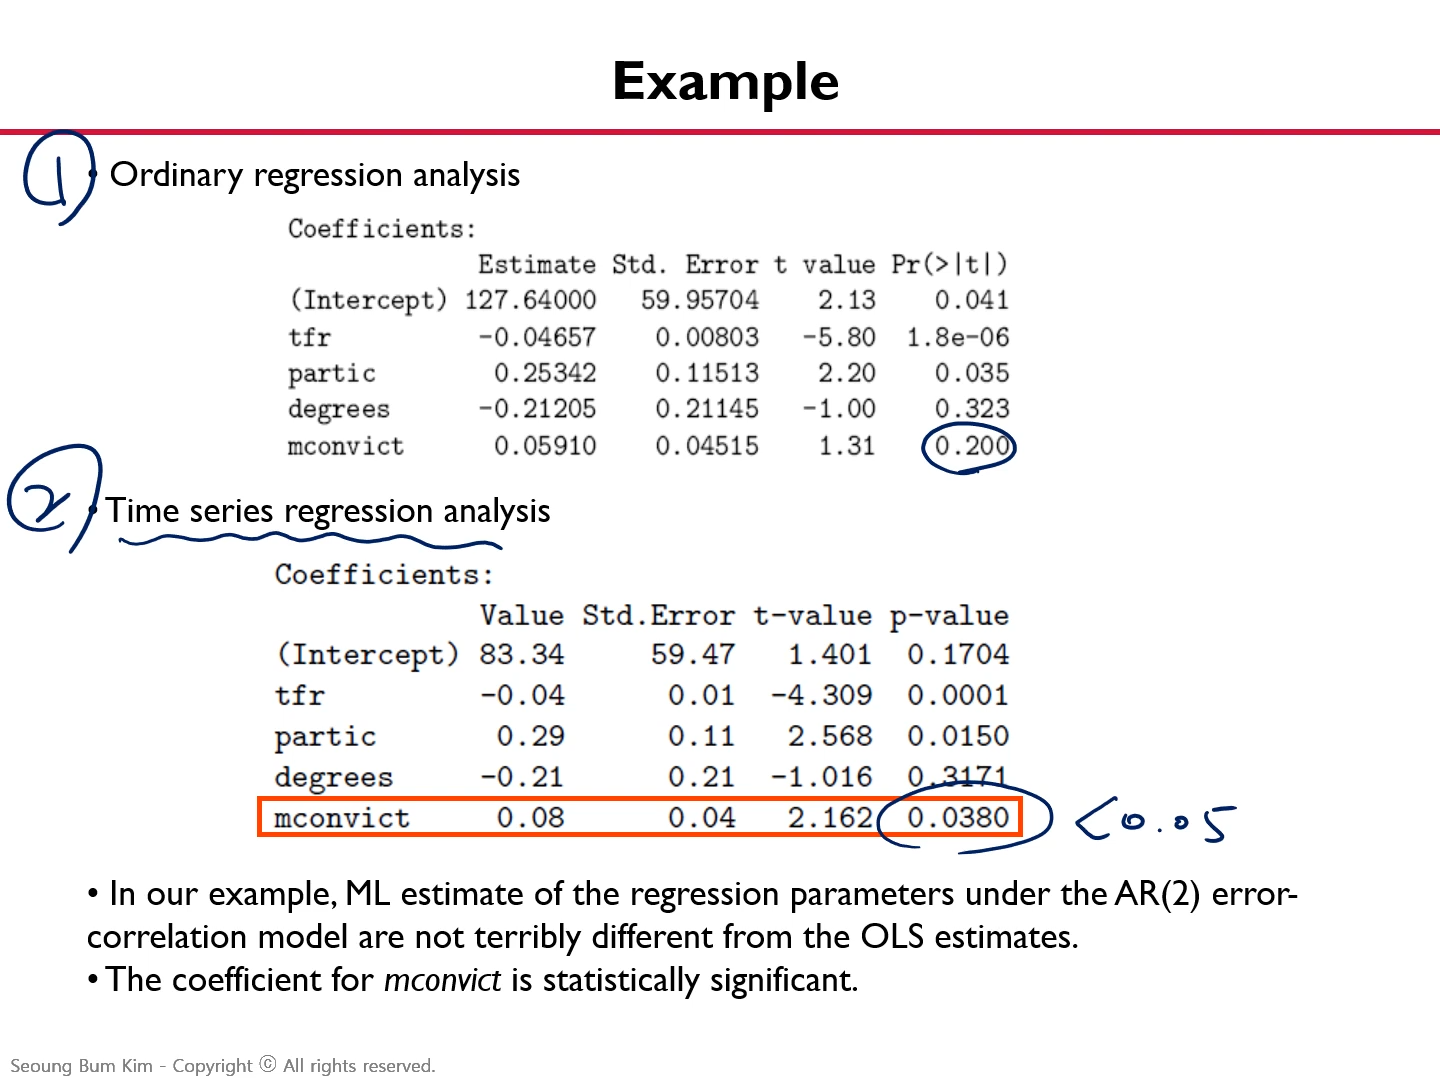
\includegraphics[width=.45\textwidth]{model_4-6}
\end{center}

\end{document}